\documentclass[11pt,a4paper]{article}
% ---------------------------------------------------------------------
%  TFPT --- Horizon and black-hole readouts of the seam constant c_3
%  Hawking/de Sitter/Unruh thermality, BH thermodynamics, Page, scrambling,
%  Nariai bound, turnaround radius, GW speed, birefringence. Honest typing.
% ---------------------------------------------------------------------
\usepackage[T1]{fontenc}
\usepackage[utf8]{inputenc}
\usepackage[english]{babel}
\usepackage{lmodern}
\usepackage[a4paper,margin=2.3cm]{geometry}
\usepackage{amsmath,amssymb,amsthm,mathtools}
\usepackage{booktabs,array,tabularx}
\usepackage{enumitem}
\usepackage{xcolor}
\usepackage[most]{tcolorbox}
\usepackage{microtype}
\usepackage[hidelinks,colorlinks=true,linkcolor=blue!55!black,urlcolor=blue!55!black]{hyperref}
\emergencystretch=3em

% ---------------------------------------------------------------------
%  tfpt_style.tex -- THE shared visual style for every TFPT document.
%  Single source for colours, status markers, marker key, the \veri
%  script reference, the tcolorbox families, and the running
%  header/footer.  \input AFTER xcolor + tcolorbox[most] + hyperref are
%  loaded (every paper loads those).  Each document sets its short
%  running title before \begin{document}, e.g.
%        \def\TFPTdoctitle{Architecture and the E8 Compiler}
%  ---------------------------------------------------------------------
\usepackage{fancyhdr}
\usepackage{etoolbox}
\usepackage{tikz}
\usetikzlibrary{positioning,arrows.meta,fit,backgrounds,calc,shapes.geometric,shapes.misc}

% ---- single-source author / version / automatic date stamp ----
% ---------------------------------------------------------------------
%  tex-artefacts/version.tex -- single source for author list, version
%  and the automatic title-page date stamp of every TFPT document.
%  \input by tex-artefacts/tfpt_style.tex, so every paper that loads the
%  shared style automatically gets:
%     \TFPTauthors   -- the author list (use as \author{\TFPTauthors})
%     \TFPTversion   -- curated semantic version (bump per release; mirror
%                       the bump in changelog.tex)
%     \TFPTrev       -- auto build revision = git commit count, injected by
%                       build.sh into tex-artefacts/version-auto.tex
%                       (gitignored); falls back to "dev" for standalone runs
%     \TFPTdatestamp -- the title-page date line: \today + version + revision
%  build.sh also writes tex-artefacts/release-version.txt (gitignored):
%     "{TFPTversion} (rev {git commit count})" for Zenodo + release tooling.
%  Bump \TFPTversion here ONCE; it then updates in all papers at the next build.
% ---------------------------------------------------------------------
\def\TFPTauthors{Stefan Hamann \and Alessandro Rizzo}
\def\TFPTversion{5.3}
\def\TFPTrev{dev}
% build.sh regenerates the line below with the live git commit count:
\InputIfFileExists{tex-artefacts/version-auto.tex}{}{}
\def\TFPTdatestamp{\today\,\textperiodcentered\,v\TFPTversion\,(rev~\TFPTrev)}


% ---- colours (canonical TFPT palette) ----
\definecolor{tfblue}{HTML}{1F4E79}
\definecolor{tfgreen}{HTML}{1E7B45}
\definecolor{tfred}{HTML}{9B2226}
\definecolor{tfgold}{HTML}{B8860B}
\definecolor{tfgray}{HTML}{555555}

% ---- status markers (simplified 4-class display system) ----
% Reader-facing markers collapse to FOUR classes.  The fine-grained per-claim
% type (Axiom / Formal / Lattice / Numerical / Identity / Physical) stays in
% verification/status_ledger.csv -- the single source of truth -- so no fidelity
% is lost; the papers just show the coarse class so a reader is not overwhelmed.
%   [E] exact / machine-proven  (identity, Lie/lattice, formalised, numerical FP)
%   [C] conditional             (physical / bridge / readout, under named hypotheses)
%   [O] open / axiom            (declared input or genuine gap)
%   [X] kill test               (falsifiable threshold)
\newcommand{\mE}{{\small\textcolor{tfgreen!70!black}{\textbf{[E]}}}}
\newcommand{\mC}{{\small\textcolor{tfgold!78!black}{\textbf{[C]}}}}
\newcommand{\mO}{{\small\textcolor{tfred!80!black}{\textbf{[O]}}}}
\newcommand{\mX}{{\small\textcolor{tfred!58!black}{\textbf{[X]}}}}
% backward-compatible aliases: the old fine-grained names now render their class,
% so any not-yet-rewritten call site (or the standalone changelog) still compiles.
\newcommand{\tI}{\mE}\newcommand{\tL}{\mE}\newcommand{\tF}{\mE}\newcommand{\tN}{\mE}
\newcommand{\tIalg}{\mE}\newcommand{\tInum}{\mE}
\newcommand{\tP}{\mC}\newcommand{\tB}{\mC}\newcommand{\tR}{\mC}
\newcommand{\tA}{\mO}
\newcommand{\tX}{\mX}

% compact marker legend, placed under a marker-bearing table
\newcommand{\markerkey}{\par\vspace{1.5pt}\noindent{\scriptsize\itshape
  \textcolor{black!58}{Marker key:\ \mE~exact / machine-proven\,$\cdot$\,%
  \mC~conditional (holds under named hypotheses)\,$\cdot$\,%
  \mO~open / axiom\,$\cdot$\,\mX~falsifiable kill test.\ \
  Per-claim fine type in \texttt{verification/status\_ledger.csv}.}}\par\vspace{2pt}}

% horizontal badge bar (place once near the front of a document)
\newcommand{\TFPTbadges}{\par\noindent
  \fcolorbox{tfgreen!55!black}{tfgreen!8}{\scriptsize\mE\,exact / machine-proven}\hfill
  \fcolorbox{tfgold!70!black}{tfgold!10}{\scriptsize\mC\,conditional}\hfill
  \fcolorbox{tfred!75!black}{tfred!8}{\scriptsize\mO\,open / axiom}\hfill
  \fcolorbox{tfred!60!black}{tfred!6}{\scriptsize\mX\,kill test}\par\vspace{3pt}}

% inline reference to the script that machine-checks a claim (see verification/)
\newcommand{\veri}[1]{\,{\footnotesize\textcolor{tfblue!70!black}{[\,\texttt{verification/#1}\,]}}}
% lightweight inline colour-mark for a bare verification-script token in running
% prose / tables, e.g. \vref{v108}, \vref{v49}/\vref{v71}.  Same blue as \veri so a
% reader instantly sees "this is a machine-checked module reference".
\newcommand{\vref}[1]{\textcolor{tfblue!72!black}{\textsf{#1}}}

% ---- tcolorbox families (one visual language across all documents) ----
% keybox  : the central claim / reading of a section (blue)
% winbox  : an established result / closure (green)
% gapbox  : an open gate / honest caveat / kill criterion (red)
% auditbox: a recorded audit fingerprint, not load-bearing (gold)
% navbox  : a light, neutral navigation / reference card (document map, etc.)
% Visual language (deliberately light): a faint tint, a thin coloured frame
% and a light title band with dark coloured title text -- NOT a heavy
% white-on-saturated-colour bar -- so a page never reads as a wall of boxes.
\newtcolorbox{keybox}[1][]{enhanced,breakable,boxrule=0.5pt,arc=1.5pt,
  colback=tfblue!4!white,colframe=tfblue!70!black,coltitle=tfblue!88!black,colbacktitle=tfblue!12!white,
  fonttitle=\bfseries\small,fontupper=\small,title={#1},left=2mm,right=2mm,top=1mm,bottom=1mm}
% non-breaking variant (front-matter cards that should never split across a page)
\newtcolorbox{keyboxnb}[1][]{enhanced,breakable=false,boxrule=0.5pt,arc=1.5pt,
  colback=tfblue!4!white,colframe=tfblue!70!black,coltitle=tfblue!88!black,colbacktitle=tfblue!12!white,
  fonttitle=\bfseries\small,fontupper=\small,title={#1},left=2mm,right=2mm,top=1mm,bottom=1mm}
\newtcolorbox{winbox}[1][]{enhanced,breakable,boxrule=0.5pt,arc=1.5pt,
  colback=tfgreen!5!white,colframe=tfgreen!65!black,coltitle=tfgreen!50!black,colbacktitle=tfgreen!14!white,
  fonttitle=\bfseries\small,fontupper=\small,title={#1},left=2mm,right=2mm,top=1mm,bottom=1mm}
\newtcolorbox{gapbox}[1][]{enhanced,breakable,boxrule=0.5pt,arc=1.5pt,
  colback=tfred!4!white,colframe=tfred!70!black,coltitle=tfred!75!black,colbacktitle=tfred!12!white,
  fonttitle=\bfseries\small,fontupper=\small,title={#1},left=2mm,right=2mm,top=1mm,bottom=1mm}
% non-breaking variants (callouts that must stay whole on one page, embedded in text)
\newtcolorbox{winboxnb}[1][]{enhanced,breakable=false,boxrule=0.5pt,arc=1.5pt,
  colback=tfgreen!5!white,colframe=tfgreen!65!black,coltitle=tfgreen!50!black,colbacktitle=tfgreen!14!white,
  fonttitle=\bfseries\small,fontupper=\small,title={#1},left=2mm,right=2mm,top=1mm,bottom=1mm}
\newtcolorbox{gapboxnb}[1][]{enhanced,breakable=false,boxrule=0.5pt,arc=1.5pt,
  colback=tfred!4!white,colframe=tfred!70!black,coltitle=tfred!75!black,colbacktitle=tfred!12!white,
  fonttitle=\bfseries\small,fontupper=\small,title={#1},left=2mm,right=2mm,top=1mm,bottom=1mm}
\newtcolorbox{auditbox}[1][]{enhanced,breakable,boxrule=0.5pt,arc=1.5pt,
  colback=tfgold!7!white,colframe=tfgold!70!black,coltitle=tfgold!45!black,colbacktitle=tfgold!16!white,
  fonttitle=\bfseries\small,fontupper=\small,title={#1},left=2mm,right=2mm,top=1mm,bottom=1mm}
\newtcolorbox{navbox}[1][]{enhanced,breakable,boxrule=0.5pt,arc=1.5pt,
  colback=tfgray!3!white,colframe=tfgray!55,coltitle=tfgray!30!black,colbacktitle=tfgray!12!white,
  fonttitle=\bfseries\small,fontupper=\small,title={#1},left=2mm,right=2mm,top=1mm,bottom=1mm}
% back-compatibility aliases (older box names map onto the canonical types)
\newtcolorbox{audbox}[1][]{enhanced,breakable,boxrule=0.5pt,arc=1.5pt,
  colback=tfgold!7!white,colframe=tfgold!70!black,coltitle=tfgold!45!black,colbacktitle=tfgold!16!white,
  fonttitle=\bfseries\small,fontupper=\small,title={#1},left=2mm,right=2mm,top=1mm,bottom=1mm}
\newtcolorbox{resbox}[1][]{enhanced,breakable,boxrule=0.5pt,arc=1.5pt,
  colback=tfgreen!5!white,colframe=tfgreen!55!black,coltitle=tfgreen!50!black,colbacktitle=tfgreen!12!white,
  fonttitle=\bfseries\small,fontupper=\small,title={#1},left=2mm,right=2mm,top=1mm,bottom=1mm}
\newtcolorbox{roadbox}[1][]{enhanced,breakable,boxrule=0.5pt,arc=1.5pt,
  colback=tfgreen!5!white,colframe=tfgreen!55!black,coltitle=tfgreen!50!black,colbacktitle=tfgreen!12!white,
  fonttitle=\bfseries\small,fontupper=\small,title={#1},left=2mm,right=2mm,top=1mm,bottom=1mm}
\newtcolorbox{intbox}[1][]{enhanced,breakable,boxrule=0.5pt,arc=1.5pt,
  colback=tfgold!7!white,colframe=tfgold!70!black,coltitle=tfgold!45!black,colbacktitle=tfgold!16!white,
  fonttitle=\bfseries\small,fontupper=\small,title={#1},left=2mm,right=2mm,top=1mm,bottom=1mm}

% ---- colour-marked display formula (load-bearing key equations) ----
% A highlighted formula line: a coloured left accent bar + faint tint, no full
% frame -- so a key equation is visually set apart from the running prose
% without becoming yet another box.  Use:  \begin{keyeq}$\displaystyle ...$\end{keyeq}
\newtcolorbox{keyeq}{blanker,breakable=false,halign=center,
  colback=tfgold!8!white,borderline west={2.4pt}{0pt}{tfgold!75!black},
  left=8pt,right=6pt,top=3pt,bottom=3pt,before skip=5pt,after skip=5pt}

% ---- running header / footer (consistent across all documents) ----
\providecommand{\TFPTdoctitle}{}
\setlength{\headheight}{14pt}
\pagestyle{fancy}
\fancyhf{}
\fancyhead[L]{\footnotesize\textcolor{tfgray}{\textit{TFPT}\,\textbullet\,\TFPTdoctitle}}
\fancyhead[R]{\footnotesize\textcolor{tfgray}{\thepage}}
\fancyfoot[L]{\scriptsize\textcolor{tfgray}{v\TFPTversion\,\textperiodcentered\,rev~\TFPTrev}}
\renewcommand{\headrulewidth}{0.3pt}
\renewcommand{\footrulewidth}{0pt}
\fancypagestyle{plain}{\fancyhf{}\renewcommand{\headrulewidth}{0pt}%
  \fancyfoot[C]{\footnotesize\textcolor{tfgray}{\thepage}}%
  \fancyfoot[L]{\scriptsize\textcolor{tfgray}{v\TFPTversion\,\textperiodcentered\,rev~\TFPTrev}}}

% ---- shared figure macros (claim stack, anchor cockpit, E8 glue, 2/3 motif, K5) ----
%  (this fragment lives in tex-artefacts/ and is \input by documents compiled from
%   the repository root, so the path is given relative to that root.)
% ---------------------------------------------------------------------
%  tfpt_figures.tex -- shared, reusable TikZ figure macros for every
%  TFPT document.  \input by tfpt_style.tex (which loads tikz + the
%  needed libraries + etoolbox).  Each macro draws a self-contained
%  centred figure; nothing is drawn until the macro is called.
%
%    \TFPTclaimstack[zone]  -- the architecture claim stack (B3); the
%                              optional zone in {axioms,anchor,compiler,
%                              sm,bridges,frontier} is highlighted.
%    \TFPTanchorcockpit      -- the anchor a=(1,1,2) cockpit (B4)
%    \TFPTeightglue          -- the D5 (+) A3 +mu4 => E8 glue (B5)
%    \TFPTmotif              -- the 2/3 motif map (B6)
%    \TFPTactionkfive        -- the K5 action-lattice mnemonic (B7)
% ---------------------------------------------------------------------

% ===== B3: the architecture claim stack =========================
\newcommand{\tfhl}[1]{\ifdefstring{\tfcur}{#1}{cbhi}{cbnl}}
\newcommand{\TFPTclaimstack}[1][none]{%
\def\tfcur{#1}%
\begin{center}
\begin{tikzpicture}[font=\footnotesize,
  cb/.style={rounded corners=2pt,inner sep=4pt,text width=118mm,align=center,minimum height=8.5mm},
  cbnl/.style={line width=0.5pt}, cbhi/.style={line width=1.5pt},
  ar/.style={-{Stealth[length=2.2mm]},tfgray,semithick}]
  \node[cb,fill=tfred!8,draw=tfred!75!black,\tfhl{axioms}] (axioms)
    {\textbf{P1}\,$c_3=\tfrac1{8\pi}$ \quad \textbf{P2}\,$g_{\mathrm{car}}=5$ \ \textcolor{tfgray}{\itshape(two inputs, [O] axioms)}};
  \node[cb,fill=tfblue!8,draw=tfblue,\tfhl{anchor},below=3.5mm of axioms] (anchor)
    {Anchor $a=(1,1,2)$:\ $e_1,e_2,e_3=4,5,2$ \ \textcolor{tfgray}{\itshape([E] exact)}};
  \node[cb,fill=tfgreen!10,draw=tfgreen!70!black,\tfhl{compiler},below=3.5mm of anchor] (compiler)
    {Discrete compiler:\ $D_5\oplus A_3+\mu_4\Rightarrow E_8$,\ $h=30$,\ $\varphi_0$ \ \textcolor{tfgray}{\itshape([E] exact)}};
  \node[cb,fill=tfgreen!7,draw=tfgreen!60!black,\tfhl{sm},below=3.5mm of compiler] (sm)
    {SM skeleton:\ three families, hypercharges, flavor matrix $R$ \ \textcolor{tfgray}{\itshape([E])}};
  \node[cb,fill=tfgold!12,draw=tfgold!80!black,\tfhl{bridges},below=3.5mm of sm] (bridges)
    {Physical bridges:\ $v_{\mathrm{geo}}$,\ $G_{\mathrm{net}}$,\ $F_{\mathrm{transfer}}$ \ \textcolor{tfgray}{\itshape([C] bridges)}};
  \node[cb,fill=tfgray!12,draw=tfgray!70!black,\tfhl{frontier},below=3.5mm of bridges] (frontier)
    {Frontier readouts:\ $\Lambda$, inflation, $\eta_B$, dark matter, QG \ \textcolor{tfgray}{\itshape([C]/[O])}};
  \draw[ar] (axioms)--(anchor); \draw[ar] (anchor)--(compiler);
  \draw[ar] (compiler)--(sm);   \draw[ar] (sm)--(bridges); \draw[ar] (bridges)--(frontier);
\end{tikzpicture}
\end{center}}

% ===== B4: the anchor cockpit ====================================
\newcommand{\TFPTanchorcockpit}{%
\begin{center}
\begin{tikzpicture}[font=\footnotesize,
  pan/.style={rounded corners=2pt,draw=tfblue!60,fill=tfblue!4,inner sep=5pt,
    text width=46mm,align=left},
  hd/.style={font=\bfseries\small,tfblue}]
  \node[pan] (e) {\textbf{elementary} $e_k(a)$\\[2pt]
     $e_1=4\to|\mu_4|$\\ $e_2=5\to g_{\mathrm{car}}$\\ $e_3=2\to|\mathbb Z_2|$\\[2pt]
     $c_3=\tfrac1{2e_1\pi}=\tfrac1{8\pi}$};
  \node[pan,right=4mm of e] (p) {\textbf{power sums} $p_n=2+2^n$\\[2pt]
     $p_0,p_1,p_2,p_3=3,4,6,10$\\ $p_1p_2p_3=240=|R(E_8)|$\\ $p_4-p_3=8=\operatorname{rank}E_8$\\
     $\Rightarrow\dim E_8=248$};
  \node[pan,right=4mm of p] (m) {\textbf{derived motifs}\\[2pt]
     $4,5,8,16,25,$\\ $30,41,120,240$\\[2pt]
     \textcolor{tfgray}{\itshape one anchor,}\\ \textcolor{tfgray}{\itshape many projections}};
  \node[hd,above=1mm of p.north] {$a=(1,1,2)$ \ \textcolor{tfgray}{\footnotesize\itshape[E]}};
\end{tikzpicture}
\end{center}}

% ===== B5: the E8 glue ===========================================
\newcommand{\TFPTeightglue}{%
\begin{center}
\begin{tikzpicture}[font=\footnotesize,
  d/.style={rounded corners=2pt,draw=tfblue,fill=tfblue!6,inner sep=4pt,align=center,text width=36mm},
  mid/.style={rounded corners=2pt,draw=tfgold!80!black,fill=tfgold!12,inner sep=4pt,align=center,text width=52mm},
  e8/.style={rounded corners=2pt,draw=tfgreen!70!black,fill=tfgreen!10,inner sep=4pt,align=center,text width=52mm,font=\bfseries},
  rt/.style={rounded corners=2pt,draw=tfgreen!55!black,fill=tfgreen!6,inner sep=3pt,align=center,text width=52mm},
  side/.style={rounded corners=2pt,draw=tfgray!55,fill=tfgray!6,inner sep=4pt,align=left,text width=34mm,font=\scriptsize},
  ar/.style={-{Stealth[length=2mm]},tfgray,semithick}]
  \node[d] (d5) {$D_5$ discriminant\\ $\mathbb Z_4$, $q=5/4$};
  \node[d,right=10mm of d5] (a3) {$A_3$ discriminant\\ $\mathbb Z_4$, $q=3/4$};
  \node[mid,below=5mm of $(d5)!0.5!(a3)$] (glue) {$\mu_4$ anti-isometry\ ($q$-sum $=2$)};
  \node[e8,below=4mm of glue] (e8) {even unimodular $E_8$ lattice};
  \node[rt,below=4mm of e8] (rt) {$240$ roots,\ rank $8$,\ $\dim=248$};
  \node[side,right=8mm of glue] (why) {\textbf{why unique?}\\ rank $8$\\ even\\ unimodular\\ positive definite};
  \draw[ar] (d5)--(glue); \draw[ar] (a3)--(glue);
  \draw[ar] (glue)--(e8); \draw[ar] (e8)--(rt);
\end{tikzpicture}\\[2pt]
{\scriptsize\itshape $D_5\oplus A_3+\mu_4\Rightarrow E_8$ --- the unique even unimodular rank-$8$ glue \ [E] exact (lattice).}
\end{center}}

% ===== B5b: the double pushout (one glue, two categories) ========
\newcommand{\TFPTdoublepushout}{%
\begin{center}
\begin{tikzpicture}[font=\footnotesize,>={Stealth[length=2mm]},
  lat/.style={rounded corners=2pt,draw=tfblue,fill=tfblue!6,inner sep=5pt,align=center,text width=34mm},
  net/.style={rounded corners=2pt,draw=tfblue!70!black,fill=tfblue!4,inner sep=5pt,align=center,text width=34mm},
  e8l/.style={rounded corners=2pt,draw=tfgold!80!black,fill=tfgold!12,inner sep=5pt,align=center,text width=34mm,font=\bfseries},
  e8n/.style={rounded corners=2pt,draw=tfgreen!70!black,fill=tfgreen!10,inner sep=5pt,align=center,text width=34mm,font=\bfseries},
  ar/.style={->,tfgray,semithick},
  lb/.style={font=\scriptsize,text=black,align=center,fill=white,inner sep=1.5pt}]
  \node[lat] (LL) at (0,2.5)   {$D_5\oplus A_3$\\[1pt]\scriptsize root lattices,\ $\mathrm{disc}=\Z_4$};
  \node[e8l] (LR) at (6.6,2.5) {$E_8$\\[1pt]\scriptsize even unimodular,\ $\det 1$};
  \node[net] (BL) at (0,0)     {$(D_5)_1\otimes(A_3)_1$\\[1pt]\scriptsize chiral nets,\ $c=8$};
  \node[e8n] (BR) at (6.6,0)   {$(E_8)_1$\\[1pt]\scriptsize holomorphic,\ $\mu$-index $1$};
  \draw[ar] (LL)--node[lb]{$+\,\mu_4$ glue}(LR);
  \draw[ar] (BL)--node[lb]{$\rtimes\,\mu_4$ extension}(BR);
  \draw[ar] (LL)--node[lb,left=-1pt]{level-$1$}(BL);
  \draw[ar] (LR)--node[lb,right=-1pt]{level-$1$}(BR);
\end{tikzpicture}\\[2pt]
{\scriptsize\itshape One operation, two categories: the order-$|\mu_4|{=}4$ glue is the lattice pushout
$D_5\oplus A_3+\mu_4\Rightarrow E_8$ \emph{and} the simple-current / anyon-condensation extension
$(D_5)_1\otimes(A_3)_1\rtimes\mu_4\cong(E_8)_1$; the square commutes. \ [E] exact.}
\end{center}}

% ===== B6: the 2/3 motif map =====================================
\newcommand{\TFPTmotif}{%
\begin{center}
\begin{tikzpicture}[font=\footnotesize,
  ex/.style={rounded corners=2pt,draw=tfgreen!70!black,fill=tfgreen!8,inner sep=4pt,align=center,text width=92mm},
  br/.style={rounded corners=2pt,draw=tfgold!80!black,fill=tfgold!12,inner sep=4pt,align=center,text width=92mm},
  ar/.style={-{Stealth[length=2mm]},tfgray,semithick}]
  \node[ex] (a) {$|\mathbb Z_2|/N_{\mathrm{fam}}=2/3$ \ \textcolor{tfgray}{\itshape(anchor ratio)}};
  \node[ex,below=3mm of a] (b) {parabolic weights $\{0,\tfrac13,\tfrac23\}=\operatorname{spec}A_0^\star$};
  \node[ex,below=3mm of b] (c) {transfer spectrum $\{1,(2/3)^6,(1/3)^6\}$,\ gap $6\log\tfrac32$};
  \node[br,below=3mm of c] (d) {Koide target $2/3$ \ \textcolor{tfgray}{\itshape(source$\to$pole bridge [C])}};
  \node[br,below=3mm of d] (e) {Nariai / horizon entropy bound $2/3$ \ \textcolor{tfgray}{\itshape([C])}};
  \draw[ar] (a)--(b); \draw[ar] (b)--(c); \draw[ar] (c)--(d); \draw[ar] (d)--(e);
\end{tikzpicture}\\[2pt]
{\scriptsize\itshape Green: exact motif ([E]).\quad Gold: physical bridge ([C]) --- the same ratio, two epistemic types.}
\end{center}}

% ===== B7: the K5 action-lattice mnemonic ========================
%  Layout: complete graph K5 (pentagon, all 10 edges) on the LEFT, the
%  Pascal-row reading list on the RIGHT, vertically centred on the graph
%  so the two blocks never overlap.
\newcommand{\TFPTactionkfive}{%
\begin{center}
\begin{tikzpicture}[font=\scriptsize]
  % --- K5 vertices on a regular pentagon, centred at the origin ---
  \foreach \i in {1,...,5}{\coordinate (k\i) at ({90+72*(\i-1)}:12mm);}
  \begin{scope}[on background layer]
    \foreach \i in {1,...,5}{\foreach \j in {1,...,5}{\ifnum\i<\j
      \draw[tfgray!55,line width=0.5pt] (k\i)--(k\j);\fi}}
  \end{scope}
  \foreach \i in {1,...,5}{\fill[tfblue!70!black] (k\i) circle (1.8pt);}
  \node[tfgray,font=\scriptsize\itshape] at (0,-1.9) {$K_5$};
  % --- reading list, anchored to the right of the whole graph, centred ---
  \node[anchor=west,align=left,inner sep=0pt] at (1.9cm,0) {%
    $\tbinom51=5$\ \ vertices --- action $x^1$ (Hubble slot)\\[1pt]
    $\tbinom52=10$\ edges --- $\Lambda$ density pair $x^{10}$\\[1pt]
    $\tbinom53=10$\ triangles --- dual sector\\[1pt]
    $\tbinom54=5$\ \ complements --- inverse sector\\[1pt]
    $\tbinom55=1$\ \ determinant --- closure};
\end{tikzpicture}\\[2pt]
{\scriptsize\itshape $K_5$ on the five carrier slots; the action powers $x^{1},x^{5},x^{10}$ are its
$\tbinom5k$ faces \ \textcolor{tfgray}{(mnemonic; the physical scale map stays [C]).}}
\end{center}}


\newcommand{\cthree}{c_3}
\newcommand{\Mbar}{\bar M_{\mathrm{Pl}}}
\newcommand{\ainv}{\alpha^{-1}_\star}
\newcommand{\Z}{\mathbb{Z}}
\newcommand{\Nfam}{N_{\mathrm{fam}}}
\setlist{itemsep=2pt,topsep=3pt}
\newcolumntype{Y}{>{\raggedright\arraybackslash}X}

\title{\vspace{-1.2cm}\textbf{TFPT --- Appendix H: the horizon unit system}\\[2mm]
\large One seam constant $\cthree=\tfrac1{8\pi}$ as the universal horizon thermal code\\
(Hawking, de Sitter, Unruh, Page, scrambling --- \emph{standard physics in seam units, not new gravity})}
\author{\TFPTauthors}\date{\TFPTdatestamp}

\def\TFPTdoctitle{Appendix~H --- Horizon Readouts}
\begin{document}
\maketitle
\vspace{-0.6cm}

\begin{keybox}[What this document is about]
A change of bookkeeping, not new gravitational physics: if gravity is the geometry-channel readout of the
seam, then \emph{all} horizons read the same boundary constant $c_3=\tfrac1{8\pi}$. This note collects the
readouts --- Hawking, de Sitter and Unruh temperature, black-hole thermodynamics, the Page time,
scrambling, the Nariai bound, $v_{\mathrm{GW}}=c$ and cosmic birefringence --- in seam units, with two
genuine compiler fingerprints ($1920=|W(D_5)|$, $|\mu_4|=4$).
\end{keybox}

\tableofcontents

% ---------------------------------------------------------------------
%  tfpt_docset.tex -- THE canonical TFPT document-set box.
%  Single source of truth for the document list; \input by the
%  introduction and every paper. Uses only universally available
%  macros (keybox + plain LaTeX math) so it compiles in every doc.
%  Each document adds its own "You are reading ..." line directly
%  after the \input.  Numbering is aligned with the file names:
%  document N == tfpt_N_*, the introduction is the entry point, and
%  R/H/O are the appendix-style companions.
% ---------------------------------------------------------------------
\begin{navbox}[The TFPT document set --- what is treated where]
\textbf{Plain language:} TFPT (Topological Fixed-Point Theory) is a small discrete compiler. Two
inputs --- the seam constant $c_3=\tfrac1{8\pi}$ and the carrier rank $g_{\mathrm{car}}=5$ --- build
$D_5\oplus A_3+\mu_4\Rightarrow E_8$ and read off the Standard-Model skeleton, the constants and the
scale grammar. The series is \textbf{the introduction plus five numbered papers and three companions},
best read in order:
\begin{enumerate}[leftmargin=2.0em,itemsep=1pt,label=\textbf{\arabic*.}]
\setcounter{enumi}{-1}
\item \texttt{introduction} --- reading guide, compiler closure, predictions, the dependency DAG and the
      single proof ledger (\texttt{verification/status\_ledger.csv}). \emph{(entry point)}
\item \texttt{tfpt\_1\_architecture\_e8} --- the two axioms, the derivation map, the EM fixed point
      $\alpha^{-1}$, the $D_5\oplus A_3+\mu_4\Rightarrow E_8$ construction, the QBL theorem chain.
\item \texttt{tfpt\_2\_standard\_model} --- the SM in one $\varphi_0$-ladder formula, flavor from
      parabolic transport (sheet diamond, dual anchor, $Q_+$ cohomology), the worked closures.
\item \texttt{tfpt\_3\_e8\_audit\_bootstrap} --- the seven $E_8$ slices as an audit raster, the cascade
      bridge, the M\"obius bootstrap.
\item \texttt{tfpt\_4\_frontier} --- honest status of $\eta_B$, $m_p/m_e$, Koide, dark matter, full QG.
\item \texttt{tfpt\_5\_redteam} --- the adversarial audit: declared attacks, what survives, what each
      reduces to, and the kill tests.
\end{enumerate}
\noindent\textbf{Companions:} \textbf{R.} \texttt{tfpt\_research\_contracts} --- the open interfaces
$(v_{\mathrm{geo}}, G_{\mathrm{net}}, F_{\mathrm{transfer}})$ as numbered contracts;
\textbf{H.} \texttt{tfpt\_horizon\_readouts} --- Appendix~H (unit-system reframe): one seam constant as
the universal horizon thermal code, the Nariai/anchor surface, the resummed seam clock;
\textbf{O.} \texttt{origin\_theory} --- why no free fundamental number remains (exact core $+$ one
honestly-typed cyclic interpretation).
\end{navbox}

\noindent\textbf{You are reading \textbf{companion~H} (Appendix~H --- Horizon Readouts).}

% ---------------------------------------------------------------------
%  tfpt_status.tex -- THE canonical "status at a glance" card.
%  Single source for the overall theory status; \input near the front
%  of every document so there is ONE status statement, not one per
%  paper.  Requires tfpt_style.tex (keybox, markers).  Detailed,
%  paper-specific status expansions live only where they belong
%  (introduction: five-questions + closure ledger; tfpt_4: frontier
%  table; tfpt_research_contracts: the contracts).
% ---------------------------------------------------------------------
\begin{keyboxnb}[TFPT status at a glance --- read this card the same way in every document]
\textbf{Two inputs, one compiler.} From the boundary constant $c_3=\tfrac1{8\pi}$ (axiom~P1) and the
five-slot carrier $g_{\mathrm{car}}=5$ (axiom~P2) --- jointly the elementary symmetric data of one anchor
$a=(1,1,2)$ --- the discrete compiler $D_5\oplus A_3+\mu_4\Rightarrow E_8$ is \emph{built}, and the
Standard-Model skeleton (gauge group, three families, hypercharges, the flavor matrix), the dimensionless
constants ($\alpha^{-1}=137.0359992$) and the scale grammar are read off as fixed points. The algebraic
core is machine-checked; physical readouts run through \emph{named bridges} whose status is typed below.
\smallskip\\
\noindent\textbf{What is closed, and what genuinely remains.} The discrete/algebraic layer is closed
(\mE); the everything-open residual reduces to \emph{three named interface problems}:
\begin{center}\small
\renewcommand{\arraystretch}{1.18}
\begin{tabular}{@{}lll@{}}
\toprule
\textbf{Interface} & \textbf{Question} & \textbf{Status} \\
\midrule
$v_{\mathrm{geo}}$ & the one metrology unit ($=1/\sqrt G=m/\mu$); No-Unit Thm: no compiler scale & primitive \mO \\
$G_{\mathrm{net}}$ & simple-current extension $(D_5)_1{\otimes}(A_3)_1{\rtimes}\langle(1,1)\rangle\cong(E_8)_1$ & \mE/\mC \\
$F_{\mathrm{transfer}}$ & one functor, four typed interfaces (Koide, $\eta_B$, axion, $m_p/m_e$) & \mC \\
\bottomrule
\end{tabular}
\end{center}
\noindent Everything carries a claim ID resolving to a row of \texttt{verification/status\_ledger.csv}
(the single source of truth); \textbf{if the text and the ledger ever disagree, the ledger wins.} The
historical labels $(U_{\mathrm{wall}},G_{\mathrm{metric}},F_{\mathrm{frontier}})$ are retained only for
ledger continuity --- the live residual is $v_{\mathrm{geo}}\oplus G_{\mathrm{net}}\oplus F_{\mathrm{transfer}}$.
\markerkey
\end{keyboxnb}

\TFPTbadges
\TFPTclaimstack[frontier]

\bigskip

\par\smallskip\noindent\textbf{Scope and honest typing.}
If gravity is the geometry-channel readout of the seam (companion note ``Seam response grammar''), then
horizons are not separate miracles --- they all read the \emph{same} boundary normaliser $\cthree=1/(8\pi)$.
This note collects the readouts. Markers: \mC\ is standard horizon physics rewritten in TFPT/seam units
(no new claim) or a search target; \mE\ is an exact compiler connection (audit-level) or a reproduced
numerical readout; \mO\ is a search target, not a result. Nothing
here is sold as new gravitational physics; it is a \emph{change of bookkeeping} that exposes shared
structure.

\begin{keybox}[Unit conventions used throughout]
Three unit systems appear; the seam factor $\cthree=1/(8\pi)$ is the same number in all of them, only the
carried dimensionful constants change:
\begin{center}\small
\renewcommand{\arraystretch}{1.25}
\begin{tabularx}{\linewidth}{@{}p{3.4cm}p{4.3cm}Y@{}}
\toprule
\textbf{system} & \textbf{convention} & \textbf{Hawking temperature} \\
\midrule
Planck & $G{=}\hbar{=}c{=}k_B{=}1$ & $T_H=\cthree/M=1/(8\pi M)$ \\
reduced Planck & $\Mbar=M_{\rm Pl}/\sqrt{8\pi}$, $\hbar{=}c{=}k_B{=}1$ & $T_H=\cthree\,\Mbar^2/M$ \\
SI & restore $G,\hbar,c,k_B$ & $T_H=\dfrac{\hbar c^3}{8\pi G k_B M}=\cthree\,\dfrac{\hbar c^3}{Gk_BM}$ \\
\bottomrule
\end{tabularx}
\end{center}
All boxed formulas below are in Planck units unless stated; the seam constant is dimensionless.
\end{keybox}

\medskip
\noindent\emph{Standard references for the formulas reframed here:} Hawking temperature and radiation
(Hawking 1975); Bekenstein--Hawking entropy (Bekenstein 1973, Hawking 1975); Page time (Page 1993);
fast scrambling $t_{\rm scr}\sim\beta\log S$ (Sekino--Susskind 2008, Maldacena--Shenker--Stanford 2016);
Nariai bound (Nariai 1950); de Sitter thermodynamics (Gibbons--Hawking 1977). \emph{Nothing below is a
new derivation of these} --- only a rewriting in the seam unit $\cthree$.

% =====================================================================
\section{The seam constant is the universal horizon temperature factor}
% =====================================================================
Every Killing horizon has $T=\hbar\kappa/(2\pi c k_B)$. Since
\[
  \boxed{\ \frac{1}{2\pi}=4\cthree,\qquad \frac{1}{8\pi}=\cthree\ }\qquad\mE,
\]
the universal factor \emph{is} the seam constant: $T_{\mathrm{hor}}=4\cthree\,\hbar\kappa/(ck_B)$. Black
holes, de Sitter and Unruh therefore share \emph{one} thermal grammar. \mC\ \veri{v8\_horizon.py}

% =====================================================================
\section{Schwarzschild thermodynamics in four $\cthree$-lines}
% =====================================================================
For a non-rotating, uncharged hole in Planck units ($G{=}\hbar{=}c{=}k_B{=}1$):
\[
  \boxed{\ T_H=\frac{\cthree}{M},\qquad S_{BH}=\frac{M^2}{2\cthree},\qquad
  P_H=\frac{\cthree}{1920\,M^2},\qquad \tau_{\mathrm{evap}}=\frac{640}{\cthree}M^3\ }\qquad\mC.
\]
Two of the constants are compiler numbers, not coincidences:
\begin{itemize}\setlength\itemsep{2pt}
\item the Hawking temperature factor is $\cthree=1/(8\pi)$ --- the same P1 boundary normaliser; \mE
\item the radiated-power denominator is $1920=|W(D_5)|$, the Weyl-group order of the $D_5$ carrier. \mE
\end{itemize}
\noindent\emph{Scope of $P_H$:} this is the idealised massless single-channel blackbody normalisation.
Greybody factors and the radiated species content shift the phenomenological evaporation coefficient; the
$\cthree$-form is the convention statement, not a general phenomenological prediction.

\begin{center}\small
\renewcommand{\arraystretch}{1.2}
\begin{tabularx}{\linewidth}{@{}p{4.2cm}YY@{}}
\toprule
\textbf{object} & \textbf{$T_H$} & \textbf{lifetime / entropy} \\
\midrule
solar-mass hole & $6.17\times10^{-8}$ K & $\tau_{\mathrm{evap}}\approx2.1\times10^{67}$ yr; $S/k_B\approx1.05\times10^{77}$ \\
PBH evaporating now ($1.7\times10^{11}$ kg) & $k_BT\approx61$ MeV & relevant for $\gamma$/$\nu$ PBH signatures \\
\bottomrule
\end{tabularx}
\end{center}

\par\smallskip\noindent\textbf{The temperature is modular; the entropy carries the scalaron.}
\veri{v208\_bh\_\allowbreak thermodynamics.py} The Hawking factor is not put in by hand: the stationary exterior
modular flow $\Delta^{it}=e^{-2\pi t K_H}$ (Bisognano--Wichmann / Tomita--Takesaki) makes the outside state
KMS at inverse temperature $2\pi$, so $T_H=\kappa/(2\pi)$ --- and that $2\pi$ \emph{is} the seam unit
$1/(4\cthree)$, reproducing $T_H=\cthree/M$ above (the seam$=$horizon modular identification ties to
$[\rho,\Lambda_\Sigma]=0$, \veri{v198\_\allowbreak modular\_\allowbreak commutator\_\allowbreak reduction.py}).
The induced $R+R^2$ scalaron then
corrects the area law to the Wald entropy
\[
  S_W=\frac{f_R\,A}{4G}=\frac{A}{4G}\Bigl(1+\frac{R_h}{3M_s^2}\Bigr),\qquad M_s=\cthree^{7/2}\Mbar,
\]
an \emph{exact} consequence of $f(R)=R+R^2/(6M_s^2)$ (\veri{v28\_gravity\_fR.py}); the leading $A/4G$ is the
$\cthree$ area law ($1/4=1/|\mu_4|$). \mE\ for the identities; the black-hole/modular identification is \mC.

% =====================================================================
\section{Page time and scrambling}
% =====================================================================
Since $S_{BH}\propto M^2$ and $\tau\propto M^3$, the Page point ($M\to M/\sqrt2$) is
\[
  t_{\mathrm{Page}}=\Bigl(1-\tfrac1{2\sqrt2}\Bigr)\tau_{\mathrm{evap}}\approx0.6464\,\tau_{\mathrm{evap}}\qquad\mC.
\]
In TFPT the Page curve is \emph{boundary recoverability}: the physical sector is OS-reconstructed and
gapped, and the recovered mutual information decays at the transfer rate,
$I(A{:}C|B)_n\sim\lambda_2^{\,n}=(2/3)^{6n}$. \textbf{This is the same operator that builds the Standard
Model:} the boundary transport spectrum is $\{1,(2/3)^6,(1/3)^6\}$ and its sub-leading eigenvalue
$\lambda_2=(2/3)^6$ is exactly the flavor-gap eigenvalue ($\Delta_{\mathrm{gap}}=-\log(2/3)^6=6\log\tfrac32$).
One boundary transport thus governs \emph{both} the SM flavor hierarchy and the horizon information recovery.
\mE\ \veri{v54\_seam\_horizon\_keystones.py}
\par\smallskip
\noindent\textbf{The recovery is a finite code (\veri{v221\_seam\_qecc.py}).} Read as a quantum channel,
this is a finite recoverability (error-correction-style) code: the code space is the carrier half-spinor
$\dim S^+=16$, the gapped transport $T$ on the cusp-weight $3$-space (deviation directions $(1,{-}1,0)$ and
the Nariai anchor $(1,1,{-}2)$) is symmetric and doubly stochastic (CPTP), and on the trace-zero subspace it
contracts with operator norm exactly $(2/3)^6$, so $\|T^n\delta\|\le(2/3)^{6n}\|\delta\|$ --- a
Knill--Laflamme-type per-step recovery bound, with a free ratio breaking it. ``Finite recoverability code''
is \mE; the holographic/Petz identification of $T$ with the Page recovery map is \mC, gated on the
Seam--Horizon theorem. The scrambling prefactor carries a $\mu_4$ signature: with
$\beta=1/T_H=8\pi M$, $\beta/2\pi=4M$, so
\[
  \boxed{\ t_{\mathrm{scr}}\sim|\mu_4|\,M\log S\ }\qquad(|\mu_4|=4)\qquad\mE\text{-audit}.
\]

% =====================================================================
\section{De Sitter and the Nariai bound from the $\Lambda$ closure}
% =====================================================================
With the action-grammar Hubble/$\Lambda$ readouts ($H_0/\Mbar=e^{-\ainv}/(2\pi\sqrt{\Omega_\Lambda})$,
$\rho_\Lambda/\Mbar^4\sim e^{-2\ainv}$), the asymptotic de Sitter horizon gives
\[
  \boxed{\ \frac{T_{dS}}{\Mbar}=16\cthree^2\,e^{-\ainv},\qquad
  S_{dS}=\frac{e^{2\ainv}}{128\cthree^4}=32\pi^4 e^{2\ainv}\approx3.32\times10^{122}\ }\qquad\mC.
\]
This is the area-law horizon capacity of the universe from $(\ainv,\cthree,H_\Lambda)$ alone. The maximal
black hole in de Sitter (Nariai) is
\[
  M_N\approx2.16\times10^{22}\,M_\odot\approx4.3\times10^{52}\,\mathrm{kg},\qquad S_N=\tfrac13 S_{dS}\qquad\mC,
\]
the absolute gravitational-capacity limit, not an observed structure.

% =====================================================================
\section{The maximal black hole is the anchor: SdS in seam units}
% =====================================================================
The Nariai limit is not just a capacity number --- written in compiler units, the entire
Schwarzschild--de~Sitter (SdS) family lands on atoms that are already load-bearing elsewhere in TFPT,
with no adjustable parameter on either side. \mE\ \veri{v101\_horizon\_anchor.py}

\par\smallskip\noindent\textbf{The defect reading: no singularity, a seam fixed point
(\veri{v209\_bh\_regular\_core.py}).} In compiler units the interior is \emph{not} a curvature blow-up but
the seam attractor: the same gapped transport whose sub-leading eigenvalue is $\lambda_2=(2/3)^6$
(\veri{v56\_unique\_attractor.py}) drives $\varphi\to\varphi_\star$ ($\mathrm d\varphi/\mathrm dt=0$), so
``$\rho\to\infty$'' is replaced by a fixed point; information returns through the same Page-recovery channel
($\lambda_2$ per step, \veri{v54\_seam\_horizon\_keystones.py}); and the end state is a holographic
Planck-scale floor ($S_{BH}=A/4$, one cell per $|\mu_4|=4$ Planck areas), not a point. \emph{Honest:} a \mC\
structural reading --- the old RN/torsion-charge metric is \emph{not} resurrected, it is superseded by the
Nariai/seam$=$horizon anchor here.

\TFPTmotif

\begin{keybox}[Nariai $=$ the anchor; the Koide $2/3$ is the entropy bound \mE\ (\veri{v101\_horizon\_anchor.py})]
With $f(r)=1-2M/r-\Lambda r^2/3$, the horizon cubic at the maximal mass
$M_N=1/(3\sqrt\Lambda)=1/(N_{\mathrm{fam}}\sqrt\Lambda)$ is, in units $1/\sqrt\Lambda$,
\[
  \boxed{\ t^3-3t+2=(t-1)^2(t+2)\ }\qquad\text{roots }(1,1,-2),
\]
with coefficients $(-3,2)=(-N_{\mathrm{fam}},|\Z_2|)$ --- and the root pattern is exactly the
\textbf{traceless projection of the anchor}: $a-\tfrac{p_1(a)}{3}\mathbf 1=-\tfrac13(1,1,-2)$ for
$a=(1,1,2)$ (compare $\chi_a=(t-1)^2(t-2)$, the anchor characteristic polynomial). Five exact companions:
\begin{itemize}\setlength\itemsep{2pt}
\item \textbf{Entropy bound $=$ the Koide branch value.} Each Nariai horizon carries $S_{dS}/3=S_{dS}/N_{\mathrm{fam}}$
and the total is $\boxed{S_{\mathrm{Nariai}}/S_{dS}=2/3=|\Z_2|/N_{\mathrm{fam}}}$ (deficit exactly $S_{dS}/3$). The
interpolation in $x=r_b/r_c$ is the closed form
$S_{\mathrm{tot}}/S_{dS}=(x^2{+}1)/(x^2{+}x{+}1)$ --- denominator $=\Phi_3(x)$, the $N_{\mathrm{fam}}$
cyclotomic --- monotone from $1$ to $2/3$ with its minimum exactly at the merge (Fig.~\ref{fig:nariai}a).
The floor admits a \emph{variation-free} one-line proof: $3(x^2{+}1)-2\Phi_3(x)=(x{-}1)^2\ge0$, so
$S_{\mathrm{tot}}\ge\tfrac23 S_{dS}$ with equality \emph{iff} $x=1$ (the Nariai merge) \mE\ (\veri{v190\_nariai\_entropy\_bound.py}).
\item \textbf{Three-sheet conservation.} The cubic is traceless with fixed $e_2$, so
$\pi\sum_i r_i^2=6\pi/\Lambda=|\Z_2|\,S_{dS}$ for \emph{every} $M$: the black hole redistributes entropy
between the two physical sheets and the virtual third root; the three-sheet total never moves.
\item \textbf{Koide-form quotient of the roots.} $Q_{\mathrm{geom}}=\sum r_i^2/(\sum|r_i|)^2$ runs
monotonically over $[\tfrac38,\tfrac12]$: pure dS gives $\tfrac12=|\Z_2|/|\mu_4|=\delta$ (the half-step),
Nariai gives $\tfrac38=p_2(a)/e_1(a)^2$ --- exactly the two nonzero $SU(4)_1$ conformal weights
(Fig.~\ref{fig:nariai}b).
\item \textbf{The mass line is a double cover.} $\operatorname{disc}_r\propto(1-3m)(1+3m)$ in
$m=M\sqrt\Lambda$: branch points $m=\pm1/N_{\mathrm{fam}}$, separation $2/3=|\Z_2|/N_{\mathrm{fam}}$, deck involution
$=$ the black-hole$\,\leftrightarrow\,$cosmological horizon swap --- the gravitational twin of the flavor
sheet $\Z_2$ and of the split $N_{\mathrm{fam}}$-linear cover $(3x{+}2)(3x{+}5)$ of the flavor sector (Fig.~\ref{fig:sdscover}).
The two branch structures share one $N_{\mathrm{fam}}$-linear ramification: the affine map
$q=\tfrac72+\tfrac{N_{\mathrm{fam}}^2}{2}m$ carries the SdS branch points $m={\pm}1/N_{\mathrm{fam}}$ onto the
flavor branch labels $\{2,5\}=\{|\Z_2|,g_{\mathrm{car}}\}$ (midpoint $7/2$). This is an exact \emph{relabeling} --- the
shared invariant is the $2/3$ ramification, not the map, which exists for any two pairs of points --- so it
is recorded as a \mC\ structural alignment, not a theorem (\veri{v191\_universal\_branch\_line.py}).
\item \textbf{Temperature lemma / orientation.} $|\kappa_b/\kappa_c|=(2x{+}1)/(x(x{+}2))>1$ for $x<1$
(equality iff $x=1$): the black-hole sheet is \emph{always} hotter, so evaporation flows \emph{away} from
the merge --- the anchor configuration is the \textbf{repeller} and the democratic endpoint the attractor,
the same orientation as the flavor flow (Koide attractor / carrier repeller, the frontier note). \emph{Audit reading.}
\end{itemize}
Completing the seam-unit table: $dM=\cthree\,\kappa\,dA$ (first law), $M=2\cthree\,\kappa A$ (Smarr),
$S\le ER/(4\cthree)$ (Bekenstein), $P_H=\cthree/(1920\,M^2)$, lifetime
$\tau=5120\pi M^3=128\,g_{\mathrm{car}}M^3/\cthree$ ($128=2^7$ the dS prefactor, $7$ the scalaron exponent;
photon/geometric-optics conventions, typed external), Kerr $A_{\mathrm{ext}}=M^2/\cthree$ with
$A_{\mathrm{ext}}/A_{\mathrm{Schw}}=1/2=1/|\Z_2|$ and $S_{\mathrm{ext}}=M^2/(4\cthree)$, and the
Bekenstein--Mukhanov--Hod area quantum $4\ln3=\ln81=\ln(N_{\mathrm{fam}}^4)=\ln(\operatorname{disc}$ of the flavor
cover$)$ (\mC\ as the QNM reading). \emph{Honest scope:} the GR identities are textbook facts; the \mE\
content is six independent landings on already-load-bearing atoms with zero free parameters. The
``carrier in the bulk'' reading (two glue chiralities $=$ two horizon sheets, ramification $=$ Nariai)
stays \mC. No new data test ($M_N$ today $\sim10^{22}M_\odot$): a structure surface, not a measurement
surface.
\end{keybox}

\begin{keybox}[The dual anchor: the inverse flavor response \emph{is} the Nariai root \mE\ (\veri{v134\_dual\_anchor.py})]
The Nariai pattern is not only the traceless anchor --- it is stored \emph{inside the flavor compiler} as a
dual invariant. For the residue/winding operators $R,L$ of the flavor sector and the anchor $a=(1,1,2)$,
\[
  \boxed{\ d:=a^\top R^{-1}=a^\top L^{-1}=\bigl(-\tfrac12,-\tfrac12,1\bigr)\ },\qquad
  d\cdot\mathbf 1=0,\quad d\cdot a=1,\quad (1,1,-2)=-2d ,
\]
i.e.\ $d=\tfrac32\bigl(a-\tfrac43\mathbf 1\bigr)$ is the \emph{normalised traceless anchor}, proportional to
the Nariai double-root pattern above. The invariance is exact and structural (Sherman--Morrison): with
$L=R+6\,\mathbf 1e_1^\top$, a covector is winding-invariant iff it annihilates $R^{-1}\mathbf
1=\tfrac14(1,1,-1)$ --- the winding deformation lives in the democratic direction $\mathbf 1$, which $d$
kills. Controls: $\mathbf 1$, $e_1$ and the torsion normal $n=(5,-9,6)$ do \emph{not} lie on the invariance
plane ($\tfrac14,\tfrac14,-\tfrac52$), so the anchor's membership is special. Together $(d,n)$ form the dual
normal pair of the flavor boundary: $d$ reads the traceless horizon structure, $n$ reads first-generation
torsion ($n^\top R=(8,0,0)$, $n^\top L=(20,0,0)$). \emph{Typing:} all identities \mE; the reading --- a
third, purely \emph{algebraic} leg of the flavor$\,\leftrightarrow\,$horizon bridge, beside the shared clock
spectrum (\veri{v126\_clock\_wall\_bridge.py}) and the entropy power law (\veri{v129\_entropy\_power\_law.py})
--- stays \mC.
\end{keybox}

\begin{figure}[h]
\centering
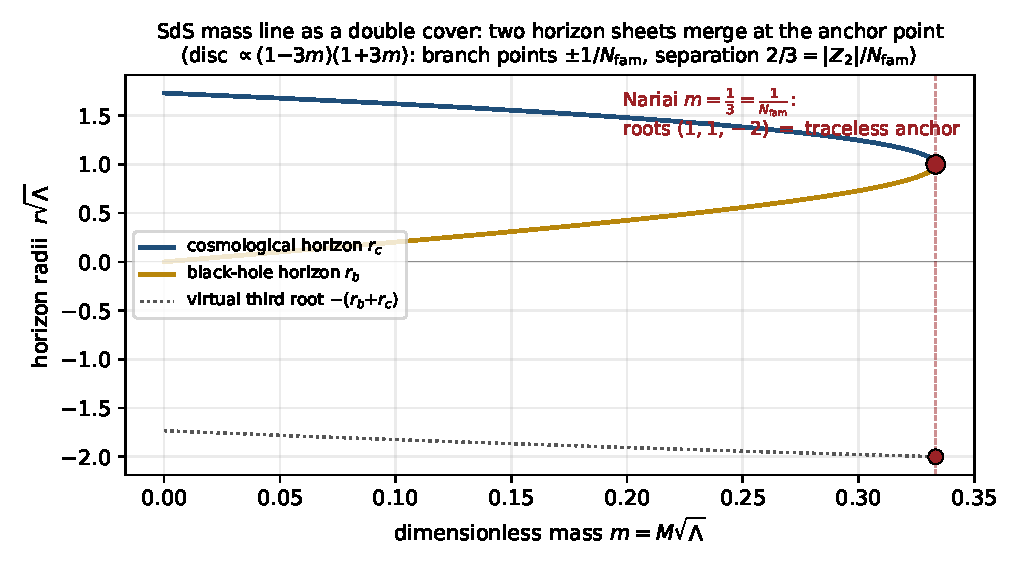
\includegraphics[width=0.78\linewidth]{figures/sds_cover.pdf}
\caption{The SdS mass line as a double cover: black-hole and cosmological horizon sheets merge at the
Nariai point $m=1/N_{\mathrm{fam}}$, where the three roots form the traceless anchor pattern $(1,1,-2)$.
\veri{v101\_horizon\_anchor.py}}
\label{fig:sdscover}
\end{figure}

\begin{figure}[h]
\centering
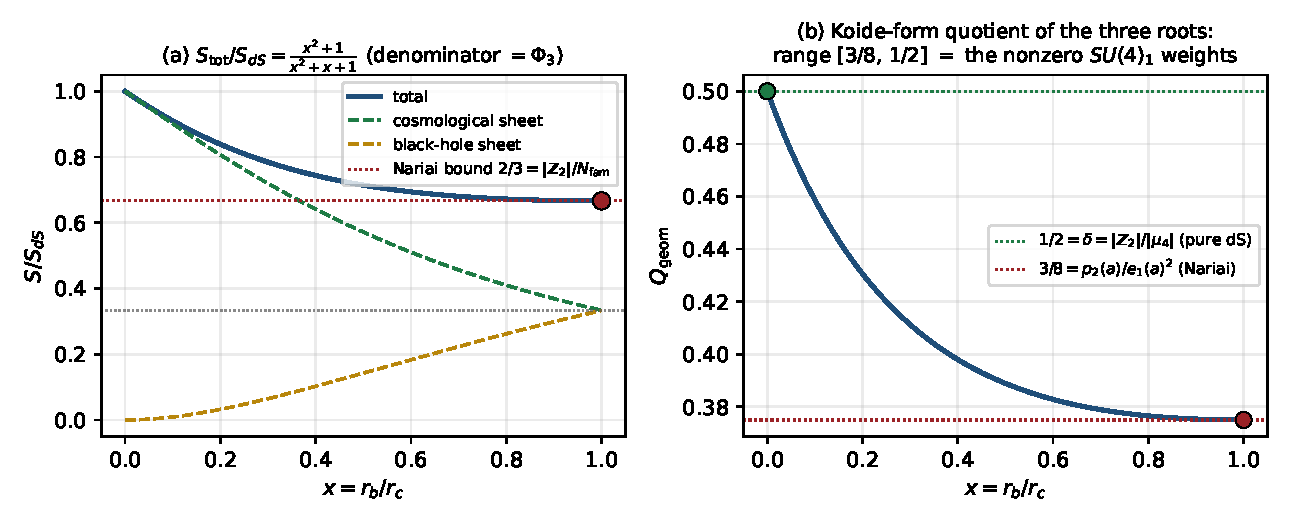
\includegraphics[width=0.94\linewidth]{figures/nariai_entropy.pdf}
\caption{(a) Total SdS entropy interpolates from $S_{dS}$ to the Nariai bound $\tfrac23 S_{dS}$ via
$(x^2{+}1)/\Phi_3(x)$. (b) The Koide-form quotient of the three roots runs exactly over the nonzero
$SU(4)_1$ weights $[\tfrac38,\tfrac12]$. \veri{v101\_horizon\_anchor.py}}
\label{fig:nariai}
\end{figure}

\begin{figure}[h]
\centering
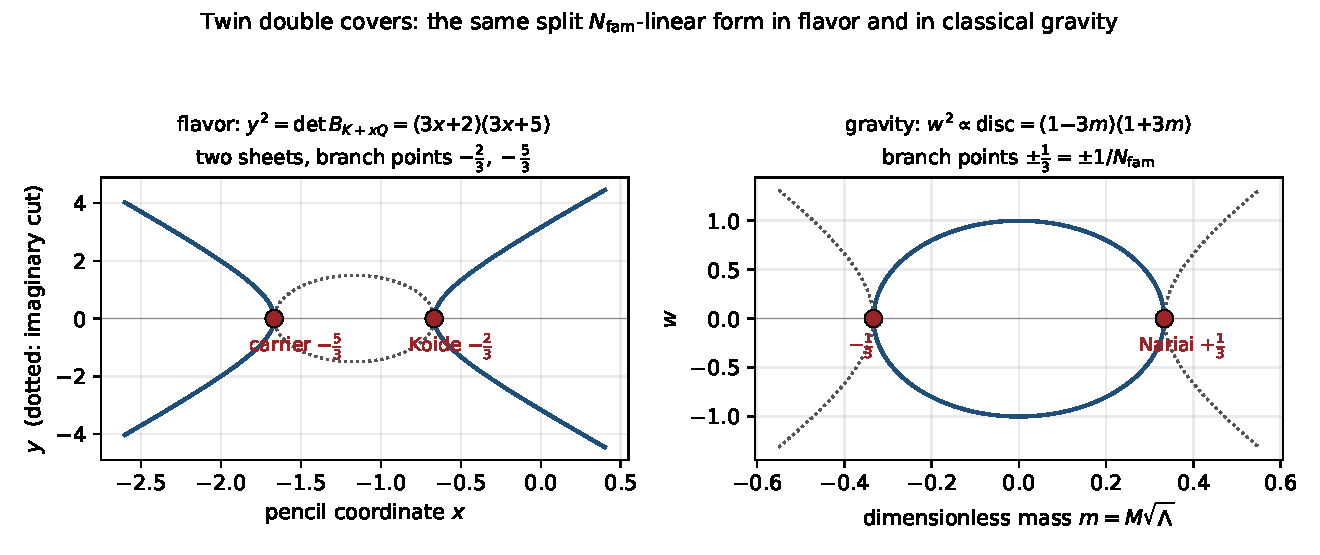
\includegraphics[width=0.94\linewidth]{figures/cover_twins.pdf}
\caption{Twin double covers: the flavor anchor-block cover $y^2=(3x{+}2)(3x{+}5)$ and the SdS
mass-line cover $w^2\propto(1{-}3m)(1{+}3m)$ share the split $N_{\mathrm{fam}}$-linear form with rational
branch points at spine-over-family values. \veri{v101\_horizon\_anchor.py}}
\label{fig:covertwins}
\end{figure}

\par\smallskip\noindent\textbf{One orientation: the anchor is the \emph{stationary repeller} in both sectors} (\mE/\mC).
The evaporation direction of the temperature lemma upgrades to exact variational structure on both
one-dimensional moduli lines (Fig.~\ref{fig:orientation}). \textbf{Flavor:} the canonical relaxation
$\dot q=(\Delta/N_{\mathrm{fam}})(q{-}2)(q{-}5)$ is the \emph{gradient flow} of the cubic potential
\[
  V(q)=-\frac{\Delta}{N_{\mathrm{fam}}}\Bigl(\frac{q^3}{3}-\frac{7}{2}q^2+10q\Bigr),\qquad
  \boxed{\ V''(2)=+\Delta,\quad V''(5)=-\Delta\ }
\]
--- the critical points are exactly the two branch points, the stationary curvatures are $\pm$the
transfer gap, the inflection sits at $q=\tfrac72=$ scalaron$/2$, and the Lyapunov rate is constant:
$d(-\ln\rho)/dt=\Delta$ exactly. \textbf{Gravity:} the SdS entropy functional has
\[
  \frac{d}{dx}\frac{S_{\mathrm{tot}}}{S_{dS}}=\frac{(x-1)(x+1)}{\Phi_3(x)^2},\qquad
  \boxed{\ \Bigl(\frac{S_{\mathrm{tot}}}{S_{dS}}\Bigr)''(1)=\frac29=\frac{|\Z_2|}{N_{\mathrm{fam}}^2}=\frac23\cdot\frac13\ }
\]
--- the Nariai/anchor point is the \emph{unique} physical stationary point, its curvature is a grammar
constant ($=$ the product of the two Nariai entropy fractions), and the temperature lemma makes the
evaporation an entropy \emph{ascent} away from it. \textbf{Orientation theorem \mE:} in both sectors the
anchor-type configuration is a stationary point of the natural functional and the dynamics flows away
from it, with grammar-constant stationary curvatures. \emph{Honest disanalogies (recorded):} the flavor
attractor is itself a branch point while the gravity attractor is the smooth endpoint; the flavor
functional is the potential of a \mC-typed relaxation while the gravity functional is the
Bekenstein--Hawking entropy --- ``one variational principle of the seam'' stays a \emph{reading} \mC, and
no open gate is touched. \veri{v102\_seam\_orientation.py}


\begin{figure}[h]
\centering
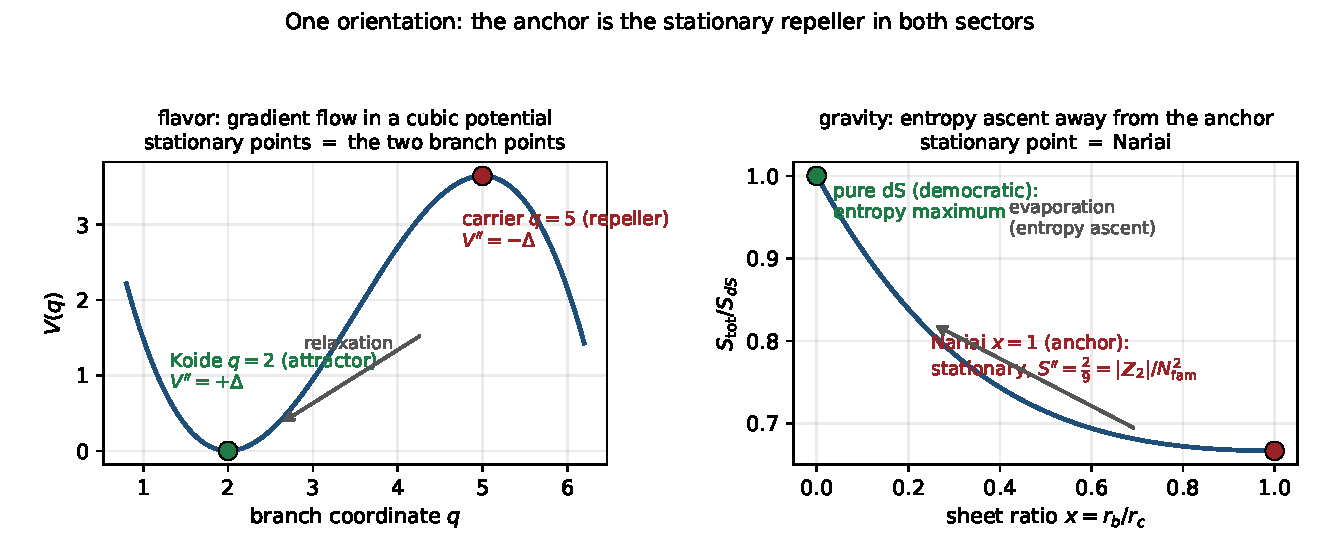
\includegraphics[width=0.94\linewidth]{figures/orientation.pdf}
\caption{The orientation theorem: the anchor configuration is the stationary repeller of the natural
functional in both sectors --- flavor (cubic potential, curvatures $\pm\Delta$) and gravity (SdS entropy,
curvature $2/9=|\Z_2|/N_{\mathrm{fam}}^2$). \veri{v102\_seam\_orientation.py}}
\label{fig:orientation}
\end{figure}

\begin{keybox}[The trisection normal form: the canonical coordinate exists \mE\ (\veri{v103\_trisection\_normal\_form.py})]
The curvature-matching question of the previous box has a closed answer. The SdS horizon cubic is
uniformized by \textbf{angle trisection}: with $r=2\cos\theta$ (units $1/\sqrt\Lambda$),
$r^3-3r=2\cos3\theta$ \emph{exactly}, so the cubic is $\cos3\theta=-3m$ --- the three horizon roots are
the three trisection branches (the $\Z_3$ rotation $=$ the triality deck, cf.\ $\operatorname{coker}Q=\Z/\Nfam$).
In the centered angle $\psi$ ($\cos\varphi=-3m$, $\psi=\varphi-\pi$; Nariai $\psi=0$, pure dS $\psi=\pi/2$,
deck $\psi\to-\psi$):
\[
  m=\frac{\cos\psi}{\Nfam},\qquad
  \boxed{\ \frac{S_{\mathrm{tot}}}{S_{dS}}=\frac43-\frac23\cos\frac{2\psi}{3}\ }
\]
--- \emph{one} cosine whose mean ($|\mu_4|/\Nfam$), amplitude and frequency (both $|\Z_2|/\Nfam$) are glue
atoms over the family count (Fig.~\ref{fig:trisection}). Three exact consequences:
\begin{itemize}\setlength\itemsep{1pt}
  \item \textbf{Canonical curvature $=$ the Koide constant to the family power:}
  $\sigma''(\psi{=}0)=\tfrac{8}{27}=(\tfrac23)^3=(|\Z_2|/\Nfam)^{\Nfam}$.
  \item \textbf{Invariant base slope:} $d\sigma/dm|_{\mathrm{Nariai}}=-\tfrac89=-\operatorname{rank}E_8/\Nfam^2$
  (coordinate-invariant, cross-checked in both coordinates; generally $-\tfrac43\sin(2\psi/3)/\sin\psi$);
  dimensionful $dS_{\mathrm{tot}}/dM|_N=-r_N/(\Nfam\cthree)$.
  \item \textbf{The bridge:} the flavor invariant is a \emph{rate}, multiplier $(2/3)^6=(2/3)^{2\Nfam}$
  per transport step; the gravity invariant is a \emph{curvature}, $(2/3)^{\Nfam}$ in the canonical angle
  --- same base $2/3=|\Z_2|/\Nfam$, exponent ratio $2=|\Z_2|$. What is still missing for a full
  identification is the gravity-side \emph{clock} (the near-Nariai evaporation generator that converts
  curvature into a rate) --- the same class of missing object as the Koide transfer generator (frontier note):
  \textbf{one clock, two known geometries}. That identification stays \mC.
\end{itemize}
\end{keybox}

\begin{figure}[h]
\centering
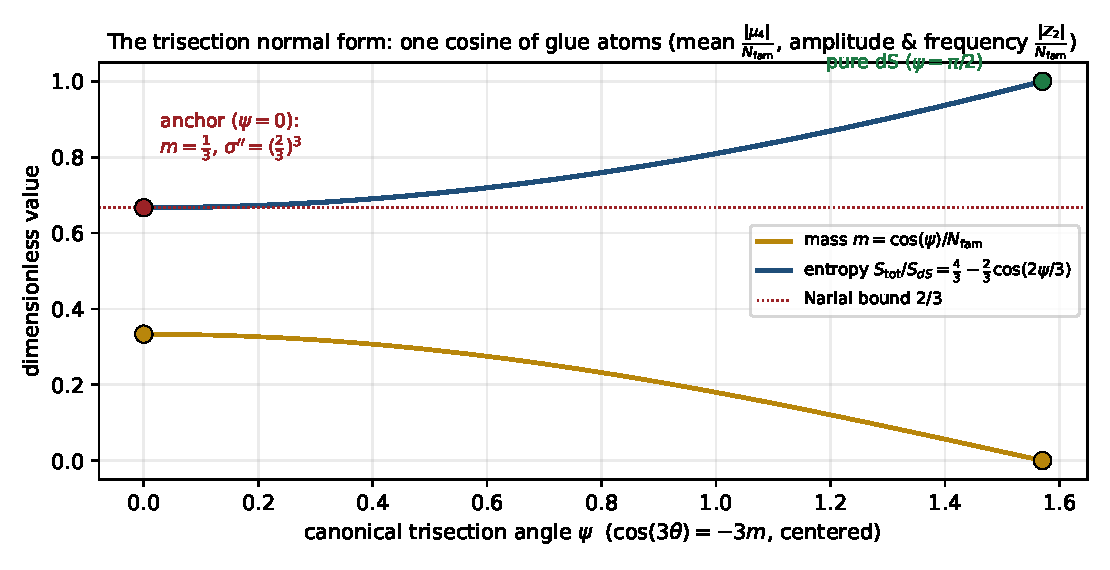
\includegraphics[width=0.86\linewidth]{figures/trisection.pdf}
\caption{The trisection normal form: in the canonical angle $\psi$ the mass and the total entropy are
pure (co)sines built from glue atoms; the anchor sits at $\psi=0$ with canonical curvature
$(2/3)^3$. \veri{v103\_trisection\_normal\_form.py}}
\label{fig:trisection}
\end{figure}

\par\smallskip\noindent\textbf{The classical clock speaks anchor --- and the honest $(2/3)$-test} (\mE/\mC).
The clock question of the previous box has a \emph{classical} half, and it is pure GR
(Ginsparg--Perry~1983; Bousso--Hawking class): linearize around the Nariai geometry
$dS_2\times S^2$. \textbf{Static pin \mE:} on the $dS_2$ static patch the function $\phi(\rho)=\rho$
satisfies $\frac{d}{d\rho}\bigl[(1-\Lambda\rho^2)\phi'\bigr]=-2\Lambda\phi$ \emph{exactly} --- and this
static mode \emph{is} the exact SdS two-horizon deformation, so the $S^2$-radius modulus mass is pinned
internally: $m^2=-2\Lambda=-|\Z_2|\Lambda$ (the Laplace-type form of the linearization is the one
external GR import, typed honestly). The Euclidean spectrum is the Ginsparg--Perry tower
$(l(l+1)-2)\Lambda$: exactly \emph{one} negative mode $-|\Z_2|\Lambda$. \textbf{The clock \mE:} in
Hubble units the homogeneous modes $\phi\sim e^{\lambda Ht}$ obey
\[
  \boxed{\ \chi_{\mathrm{clock}}(\lambda)=\lambda^2+\lambda-2=(\lambda-1)(\lambda+2)\ }
\]
--- \textbf{the anchor quadratic}: eigenvalues $\{1,-2\}$ $=$ the distinct anchor roots, and the Nariai
cubic factors as $(t-1)^2(t+2)=(t-1)\cdot\chi_{\mathrm{clock}}(t)$. The anchor thus appears a
\emph{third} time: as configuration roots, as the curvature base, and as the spectrum of the linearized
clock. The horizon split is linear in the canonical angle with coefficient $1/\sqrt{\Nfam}$, and the
entropy deviation grows at exactly $2H=|\Z_2|\times$Hubble. \textbf{Honest $(2/3)$-test \mC:} the
classical clock eigenvalues are \emph{integers}, not $(2/3)$-powers --- the $(2/3)$-powers stay in the
functional (curvature $(2/3)^{\Nfam}$). The conversion curvature$\to$rate at one loop (quantum
(anti-)evaporation) remains external QFT input: the bridge to the flavor rate $(2/3)^{2\Nfam}$ is
\emph{not} closed here. The seam variational principle now has exactly \emph{one} missing object: the
quantum clock. \veri{v104\_nariai\_clock.py}


\par\smallskip\noindent\textbf{The quantum-clock target, made quantitative} (\mE/\mC).
Instead of guessing the quantum clock, its job description can be pinned exactly. \textbf{(1) The
classical clock already lives on the cusp ladder \mE:} across the physical Ginsparg--Perry modes
($l=0$: $(\lambda{-}1)(\lambda{+}2)$; $l=1$: $\lambda(\lambda{+}1)$) the decay exponents are
\[
  \boxed{\ \{0,-1,-2\}=-\operatorname{Spec}(V)=-\Nfam\times\text{cusp weights}\ }
\]
--- exactly the grading that carries the transfer operator's eigenspaces (Papers~2/6); the $l\ge2$ modes
are damped oscillations with $\operatorname{Re}\lambda=-\tfrac12=-\delta$ (audit). \textbf{(2) The exact
target \mE:} the transfer rates $\{0,\Delta,6\ln3\}$ are \emph{not} weight-linear ---
$\mathrm{rate}(2)/\mathrm{rate}(1)=\log_{3/2}3=1+\log_{3/2}2=2.7095$, with the exact identity
$(1/3)^6=\bigl((2/3)^6\bigr)^{\log_{3/2}3}$: \emph{the quantum clock must bend the weight-linear spectrum
by $\log_{9/4}3=1.35476$ per weight step}. \textbf{(3) Coupling landscape \mE:} the dimensionless clock
coupling $\kappa=(c/24\pi)(\Lambda/\bar M_{\mathrm{Pl}}^2)$ with $c=8$ is $7.6\times10^{-122}$ at the
cosmological Nariai (hopeless) and $\kappa=1/(3\pi)=0.106$ at seam curvature --- the only regime where an
$O(0.35)$ bend is reachable, and it is borderline non-perturbative: one-loop linear response cannot fix
the bend; an $O(1)$ resummation or an exact seam construction is required. \emph{Status \mC:} R1 is
sharpened from ``find a clock'' to ``produce the bend $\log_{3/2}3$ on the cusp ladder at coupling
$O(1/3\pi)$''. Nothing is fitted; the identification stays open. \veri{v107\_quantum\_clock\_target.py}


\par\smallskip\noindent\textbf{The resummed clock: the bend has a closed form} (\mE/\mC).
The ``bend'' is not an exotic target --- the frozen transfer spectrum \emph{is} a resummed logarithm.
\textbf{(1) Spectrum reading \mE:} the eigenvalues $\{1,(\tfrac23)^6,(\tfrac13)^6\}$ are exactly
\[
  \boxed{\ \lambda_n=\Bigl(1-\frac n{\Nfam}\Bigr)^{p_2},\qquad n=0,1,2\ }
  \qquad(p_2=6=|R^+(A_3)|),
\]
so the clock has the closed form $\mathrm{rate}(n)=-p_2\ln(1-n/\Nfam)$ --- it reproduces
$\{0,\Delta,6\ln3\}$, and the \vref{v107} bend $\log_{3/2}3$ becomes a one-line consequence. \textbf{(2) The
linearisation carries the sheet \mE:} $\mathrm{rate}(n)=|\Z_2|\,n+\tfrac{n^2}3+\tfrac{2n^3}{27}+\cdots$
--- the one-loop term has slope exactly $|\Z_2|=2$ relative to the \emph{integer} classical
Ginsparg--Perry clock $\{0,-1,-2\}$: the quantum clock is the sheet-doubled classical clock plus the
geometric tail $\sum_k(n/N)^k/k$. \textbf{(3) The wall at $\Nfam$ \mE:} $\mathrm{rate}\to\infty$ as
$n\to\Nfam$ --- the resummed logarithm has a pole at the family count, so the cusp ladder \emph{must}
end at $n=\Nfam-1=2$: the three-level transfer spectrum is forced by the clock itself. \emph{R1
re-sharpened \mC:} the semiclassical job is now ``derive $-p_2\ln(1-n/\Nfam)$ from the near-Nariai
one-loop at $\kappa=1/(3\pi)$'' --- a closed-form target, with the linear-response slope $|\Z_2|$ as
its first checkpoint. All spectra frozen (\vref{v54}/\vref{v69}/\vref{v95}/\vref{v104}/\vref{v107}); nothing fitted. \veri{v124\_resummed\_clock.py}


\par\smallskip\noindent\textbf{The clock and the wall share a spectrum} (\mE/\mC).
Both ends of the resummed clock connect to established exact objects. \textbf{(1) The weights are the
parabolic weights \mE:} the arguments $n/\Nfam=\{0,\tfrac13,\tfrac23\}$ of the resummed logarithm are
\emph{exactly} $\operatorname{spec}A_0^\star$ --- the spectrum of the exact $(U_{\mathrm{wall}})$
residue (research contracts):
\[
  \boxed{\ \lambda_n=(1-\alpha_n)^{p_2},\qquad \alpha_n\in\operatorname{spec}A_0^\star=\{0,\tfrac13,\tfrac23\}\ }
\]
--- the horizon clock and the flavor wall share their spectrum through the complement map
$\alpha\mapsto1-\alpha$. \textbf{(2) Checkpoint 1 passes classically \mE:} the clock's linear
coefficient $p_2/\Nfam=2=|\Z_2|$ \emph{equals} the established classical entropy-deviation rate
$2H=|\Z_2|\times$Hubble (\vref{v104}) --- the slope-$2$ linear response is already the classical entropy
rate; the genuinely \emph{quantum} content of R1 isolates to the geometric tail
$\sum_{k\ge2}\alpha^k/k$. \textbf{(3) The determinant is the entropy curvature \mE:}
$\det(\mathbf1-A_0^\star)=\tfrac29=|\Z_2|/\Nfam^2$ --- exactly the gravity entropy curvature at the
anchor (\vref{v102}), a fourth independent appearance; $\operatorname{tr}(\mathbf1-A_0^\star)=2=|\Z_2|$,
$\det A_0^\star=0$. \emph{R1 re-targeted \mC:} derive ``rate $=-p_2\ln(1-\alpha)$'' with $\alpha$ the
Mehta--Seshadri parabolic weight --- first order classical, tail quantum: \textbf{one spectrum, two
gates, one object $A_0^\star$}. \veri{v126\_clock\_wall\_bridge.py}


\par\smallskip\noindent\textbf{The clock is a log-determinant: the tail is the ring (RPA) resummation} (\mE/\mC).
The ``$O(1)$ resummation'' demanded by \vref{v107} is now \emph{typed}. For a rank-one insertion $P$
($\operatorname{tr}P^k=1$), $-\ln\det(\mathbf1-\alpha P)=-\ln(1-\alpha)=\sum_k\alpha^k/k$, so the
resummed clock is exactly
\[
  \boxed{\ \mathrm{rate}=-p_2\,\operatorname{Tr}\ln(\mathbf1-\alpha P)\ }
\]
--- $p_2=6$ \emph{identical} one-loop ring (RPA) towers, \textbf{one per hexagon site} ($=$ positive
root of $A_3$), with coupling $\alpha$ $=$ the parabolic weight. \emph{Ring ladder \mE:} the $k{=}1$
ring is the \emph{classical} term ($6\alpha=|\Z_2|n$, the \vref{v104}/\vref{v126} entropy rate); the $k{=}2$ ring is
the first quantum correction ($\tfrac13$ at weight $1$); the partial sums converge to
$\{\Delta,6\ln3\}$ monotonically from below. \emph{Coupling cross-link \mE\ (audit):} the established
seam coupling is $\kappa=\tfrac c{24\pi}=\tfrac8{24\pi}=\tfrac1{3\pi}=\alpha_1/\pi$ --- the
\emph{first parabolic weight over $\pi$}. \emph{The wall \mE:} the ring series diverges at
$\alpha\to1$ ($n\to\Nfam$) --- the \vref{v124} wall is the standard RPA instability. \emph{R1 final form
\mC:} show that the near-Nariai one-loop effective action of the seam mode, with insertion $=$
parabolic weight and multiplicity $p_2$, is this ring sum --- ``\textbf{the seam clock is the RPA
determinant of one mode on six sites}''. The resummation type is identified; the derivation itself
remains open.
\smallskip\\
\noindent\emph{Where the six sites live (\veri{v128\_graded\_hull.py}):} the Ginsparg--Perry $l=1$
sector --- the \emph{zero modes} $\lambda\in\{0,-1\}$ of the classical clock (\vref{v104}/\vref{v107}) --- has
$2l+1=3$ modes, and sheet doubling gives $2\times3=6=p_2$ \mE: the ring multiplicity equals the
sheet-doubled zero-mode count. \mC\ reading (recorded): zero modes are exactly the modes that force
nonperturbative resummation in de Sitter one-loop physics --- the natural home of the six RPA towers. \veri{v127\_ring\_resummation.py}


\par\smallskip\noindent\textbf{The clock is an entropy power law} (\mE/\mC).
What the resummation argument $1-n/\Nfam$ \emph{is} physically: the three established Nariai entropy
levels (\vref{v101}) are $S/S_{dS}\in\{1,\tfrac23,\tfrac13\}$ (pure dS; two-horizon total; single horizon ---
deficit $S_{dS}/3$ per step) --- exactly the complementary cusp weights. Hence \mE:
\[
  \boxed{\ \lambda_n=\Bigl(\frac{S_n}{S_{dS}}\Bigr)^{p_2},\qquad
  \mathrm{rate}(n)=p_2\ln\frac{S_{dS}}{S_n}\ }
\]
--- the transfer eigenvalues are the \emph{entropy fractions to the hexagon power}; the rates are
hexagon-weighted log-entropy deficits. \emph{The coupling is the entropy deficit \mE\ (triple
identity):} $\alpha=n/\Nfam$ $=$ the Mehta--Seshadri parabolic weight (\vref{v115}/\vref{v126}) $=$
$1-S_n/S_{dS}$ $=$ $\Delta S_n/S_{dS}$ --- the RPA insertion strength is the fractional entropy
deficit; the coupling is not a free parameter in \emph{any} of its three readings. \emph{Orientation
\mE:} weight $0\leftrightarrow$ pure dS (maximal entropy, stationary attractor), weight
$2\leftrightarrow$ single horizon (fastest decay) --- the established repeller$\to$attractor flow.
\emph{R1, thermodynamic form \mC:} derive $\Gamma_n\propto(S_n/S_{dS})^{p_2}$ from the near-Nariai
one-loop --- a Gibbons--Hawking-type entropy power law with exponent $=$ the hexagon size (audit:
$p_2=6=2h$ reads as the two-point form of a weight $h=3=\Nfam$ operator; recorded, not claimed).
\smallskip\\
\noindent\emph{The Born square (\veri{v130\_born\_square.py}):} the weight audit is now \emph{derived}
from mode counting \mE. In the standard collective-coordinate treatment each zero mode contributes a
moduli factor $\propto S^{1/2}$, so with $n_{\mathrm{zero}}=6$ the transition \emph{amplitude} scales
as $A\sim(S/S_{dS})^{3}$ and the \emph{probability} is its Born square $\Gamma=|A|^2=(S/S_{dS})^{6}$:
\[
  \boxed{\ h=\tfrac{n_{\mathrm{zero}}}2=3=\Nfam,\qquad p_2=2h\ \text{(the Born rule)}\ }
\]
--- and the $3$ is the dimension of the $l{=}1$ eigenspace $=$ the number of \emph{proper conformal
Killing vectors of $S^2$} (the classic near-Nariai zero modes, Ginsparg--Perry/Bousso--Hawking class),
while the $\times2$ is the \emph{horizon pair} $=$ the SdS mass-line deck (\vref{v101}). The same $3$ counts
the generations and the sphere's conformal directions. \emph{Residue \mC:} justify the per-zero-mode
$S^{1/2}$ normalisation on the Nariai instanton for exactly these six modes --- a textbook-class
computation; no exotic object remains in R1.
\smallskip\\
\noindent\emph{The measure is the area (\veri{v131\_measure\_is\_area.py}):} the geometric core of
that normalisation is exact \mE: on $S^2(r)$ the $L^2$ norm of \emph{each} of the three normalised
$l{=}1$ harmonics is
\[
  \boxed{\ \|Y_{1m}\|^2=r^2=\frac{A}{4\pi}\ }
\]
(all three integrated exactly) --- the zero-mode norm \emph{is} the horizon area, hence the entropy.
The collective-coordinate Jacobian per mode is the mode norm $\sim S^{1/2}$ (standard change of
variables), so: norm $=$ area $\to$ Jacobian $=S^{1/2}$ $\to$ six modes $\to$ amplitude $S^3$ $\to$
Born $\to$ $S^6$ --- every exponent factor carries a derivation-level origin. The $4\pi$ is the same
Gauss--Bonnet primitive that builds $\cthree=\tfrac12(4\pi)^{-1}$, and it \emph{cancels} in all
ratios --- exactly why the clock sees only entropy fractions. \emph{The last step \mC:} show
$\det'_n/\det'_{dS}=1+O(\text{deficit})$ (non-zero-mode determinant cancellation; same local
near-Nariai geometry). \veri{v129\_entropy\_power\_law.py}
\smallskip\\
\noindent\emph{The cancellation, exact within the family (\veri{v144\_detratio\_family.py}):} that step
is now \emph{derived} in the within-family sense \mE. The traceless SdS cubic forces
\[
  \boxed{\ r_b\,r_c=1-\frac{\Delta^2}{3}\quad(\Delta=r_b-r_c\ \text{the horizon split; exact, no higher
  corrections})\ }
\]
($e_2$-rigidity), and with the \vref{v132} anomaly $\zeta(0)|_{\det'}=-\tfrac23$ per sphere the
two-sphere non-zero-mode determinant ratio against Nariai is the closed form
$\det'_n/\det'_N=(1-\Delta^2/3)^{4/3}$: \textbf{no first-order term in the split} --- the hoped-for
cancellation is a consequence of $e_2$-rigidity plus the established anomaly, not an assumption. In
deficit form, $\varepsilon=1-c=\tfrac38\Delta^2+O(\Delta^4)$ gives
$\det'_n/\det'_N=1-\tfrac{32}{27}\varepsilon+O(\varepsilon^2)$ with
$\tfrac{32}{27}=|\mu_4|(\tfrac{|\Z_2|}{\Nfam})^3$ (the \vref{v103} canonical curvature times the glue
order; audit-typed). \emph{Honest scope \mC:} the finite-weight comparison
($S_n/S_{dS}\in\{1,\tfrac23,\tfrac13\}$) still runs through the \vref{v132}/\vref{v133} budget --- a naive
global-rescaling reading would shift the Born exponent $6\to\tfrac{14}3$ (not an atom), so the absorption
must proceed via the Hubble-unit conversion; the frozen transfer spectrum is untouched, and the remaining
\mC\ now has its obstruction stated sharply.
\smallskip\\
\noindent\emph{The clock is a Gaussian zero-mode integral (\veri{v147\_clock\_gaussian.py}):}
the \vref{v127} typing job is discharged at the model level, and the bend is det$'$-clean \mE. For
$p_2$ Gaussian zero modes whose per-mode variance scales by $(1-\alpha)$ --- \emph{forced} by
norm $=$ area (\vref{v131}) --- the Born-squared partition ratio is exactly $(1-\alpha)^{p_2}$, i.e.\
$\mathrm{rate}=-p_2\ln(1-\alpha)$, and the $\ln$ series \emph{is} the ring sum $p_2\sum_k\alpha^k/k$
term by term. Sharper still: the two quantum weights $n=1,2$ are bookkeeping levels of \emph{one}
Euclidean geometry (Nariai $S^2{\times}S^2$, \vref{v101}), so $\det'_1=\det'_2$ \emph{identically} ---
\textbf{the bend $\log_{3/2}3$ (the \vref{v107} target) carries no determinant correction at all}. The
single across-topology step is the $\alpha=0$ reference (round dS vs Nariai), exactly where the
\vref{v132}/\vref{v133} budgets and the \vref{v144} obstruction live; its classical side is already
matched (\vref{v126}: slope $2=|\Z_2|$). \emph{What stays \mC:} the measure identification
(``the gravitational near-Nariai zero-mode measure \emph{is} this Gaussian model'') and the reference
normalisation --- structure, spectrum, bend and ring typing are exact.


\par\smallskip\noindent\textbf{The det-ratio anomaly is the Koide constant} (\mE/\mC).
The det-ratio question acquires its first \emph{exact} invariant. The Ginsparg--Perry sphere operator
on the unit $S^2$ is $L=-\Delta-2$ (the $-2=-|\Z_2|$ is the \vref{v104} modulus mass), with eigenvalues
$(l{+}2)(l{-}1)$ and kernel the three $l{=}1$ zero modes. Its heat coefficient is made of atoms \mE:
$a_1=\tfrac R6-E=\tfrac13+2=\tfrac1{\Nfam}+|\Z_2|=\tfrac73$, and the scaling anomaly of the
non-zero-mode determinant is
\[
  \boxed{\ \zeta(0)\big|_{\det'}=a_1-\dim\ker=\tfrac73-3=-\tfrac23=-\frac{|\Z_2|}{\Nfam}\ }
\]
--- confirmed independently by numerical continuation of the heat trace ($\sim10^{-7}$): \textbf{the
det-ratio anomaly is the Koide constant}, the eighth appearance of $2/3$ and the first as a
\emph{spectral} anomaly. \emph{Consequence \mE:} $\det'(cL)=c^{\zeta(0)}\det'(L)$ --- the determinant
ratio between configurations is \emph{not} automatically $1$; the $S^2$-sector share of the scaling
budget is exactly $-\tfrac23$ per Hubble-unit conversion, while the dimensionless tower itself is
configuration-independent (pure-number GP spectrum). \emph{The budget statement \mC\ (the remaining
step, made precise):} show the \emph{full} $\zeta(0)$ budget of the 4d Nariai fluctuation problem
($dS_2$ $+$ gauge/ghost $+$ this $S^2$ sector) vanishes or is absorbed into the established power law
--- the $S^2$ share is pinned exactly; nothing is claimed about the total. \veri{v132\_detratio\_anomaly.py}


\par\smallskip\noindent\textbf{The zeta budget: the reduced route carries the anchor ratios} (\mE/\mC).
Euclidean Nariai is $S^2\times S^2$ --- the temporal sector continues to the \emph{same} unit sphere,
so both candidate determinant routes are exactly computable. \emph{(i) The reduced route \mE:} each
2d sector carries the \vref{v132} operator with $\zeta(0)|_{\det'}=-\tfrac23$; the two sectors give
\[
  \boxed{\ \text{budget}_{\mathrm{red}}=-\tfrac23-\tfrac23=-\tfrac43=-\frac{e_1}{p_0}\ \text{(minus
  the seed gain)}\ }
\]
--- the per-sector share and the total are \emph{two of the three \vref{v119} anchor-ratio triad values};
the six zero modes split $3+3$ across the two spheres: the sheet doubling \emph{is} the two-sphere
structure of Euclidean Nariai ($=$ the horizon pair, \vref{v101}). \emph{(ii) The naive 4d route \mE:} with
the standard $S^2$ heat expansion $1/t+\tfrac13+t/15$ and the symmetric split, $a_2(4d)=
(\tfrac43)^2+2\cdot\tfrac9{10}=\tfrac{161}{45}$, six zero modes, $\zeta(0)|_{\det',4d}=
\tfrac{161}{45}-6=-\tfrac{109}{45}$ --- \emph{no} anchor-atom reading. \emph{(iii) Route
discrimination \mC:} the budget computation structurally favours the \textbf{reduced seam reading}
(pure anchor-ratio anomalies), consistent with the theory's 2d-seam architecture throughout ---
route-selection evidence, not proof. \emph{Remaining \mC:} the graviton/ghost shares on $S^2\times
S^2$ (Volkov--Wipf class, external standard) --- a finite list of known heat coefficients. \veri{v133\_zeta\_budget.py}


\par\smallskip\noindent\textbf{The Volkov--Wipf firewall: the external edge is two copies of the reduced budget} (\mE/\mC).
The ``finite list'' above is now \emph{filled in externally}. For the full one-loop graviton path
integral on $S^2\times S^2$ the log-coefficient is (arXiv:2506.02142, Table~4.1, agreeing with
Volkov--Wipf, Nucl.\ Phys.\ B582 (2000) 313):
\[
  \alpha_{\mathrm{bulk}}=\tfrac{22}{45},\qquad \alpha_{\mathrm{edge}}=-\tfrac83,\qquad
  \alpha_{\mathrm{PI}}=-\tfrac{98}{45}
\]
(no anchor atom; the difference to the reduced budget is $-\tfrac{38}{45}$ with $38=2\cdot19$).
The structural finding: the external \emph{edge} factor consists of \textbf{two identical copies} (one
per horizon), and
\[
  \boxed{\ \alpha_{\mathrm{edge}}=-\tfrac83=2\times\bigl(-\tfrac43\bigr)\ }
\]
--- the per-copy magnitude $\tfrac43=e_1/p_0$ is \emph{exactly} the reduced seam budget above (the seed
gain; $-\tfrac23$ per sector). The TFPT reduced route lands on the \textbf{edge sector} of the external
bulk/edge split; the bulk ($\tfrac{22}{45}$) is the ideal graviton gas, which the seam clock does not
contain; two copies $=$ the horizon pair $=$ the sheet doubling (\vref{v101}; the $3{+}3$ zero-mode split).
\emph{Typing decision \mC\ (recorded):} R1 $=$ the reduced zero-mode/RPA seam clock $=$ an edge-sector
object; the full 4d Volkov--Wipf determinant is the \emph{gravity firewall} (its $-\tfrac{98}{45}$ is
absorbed in the $\mu_0/(\Lambda G)^3$ normalisation), not a TFPT atom. Per-copy sign/orientation (the
edge factor enters inverted) and the Lorentzian edge-mode reading stay \mC. \veri{v138\_vw\_firewall.py}


\begin{figure}[h]
\centering
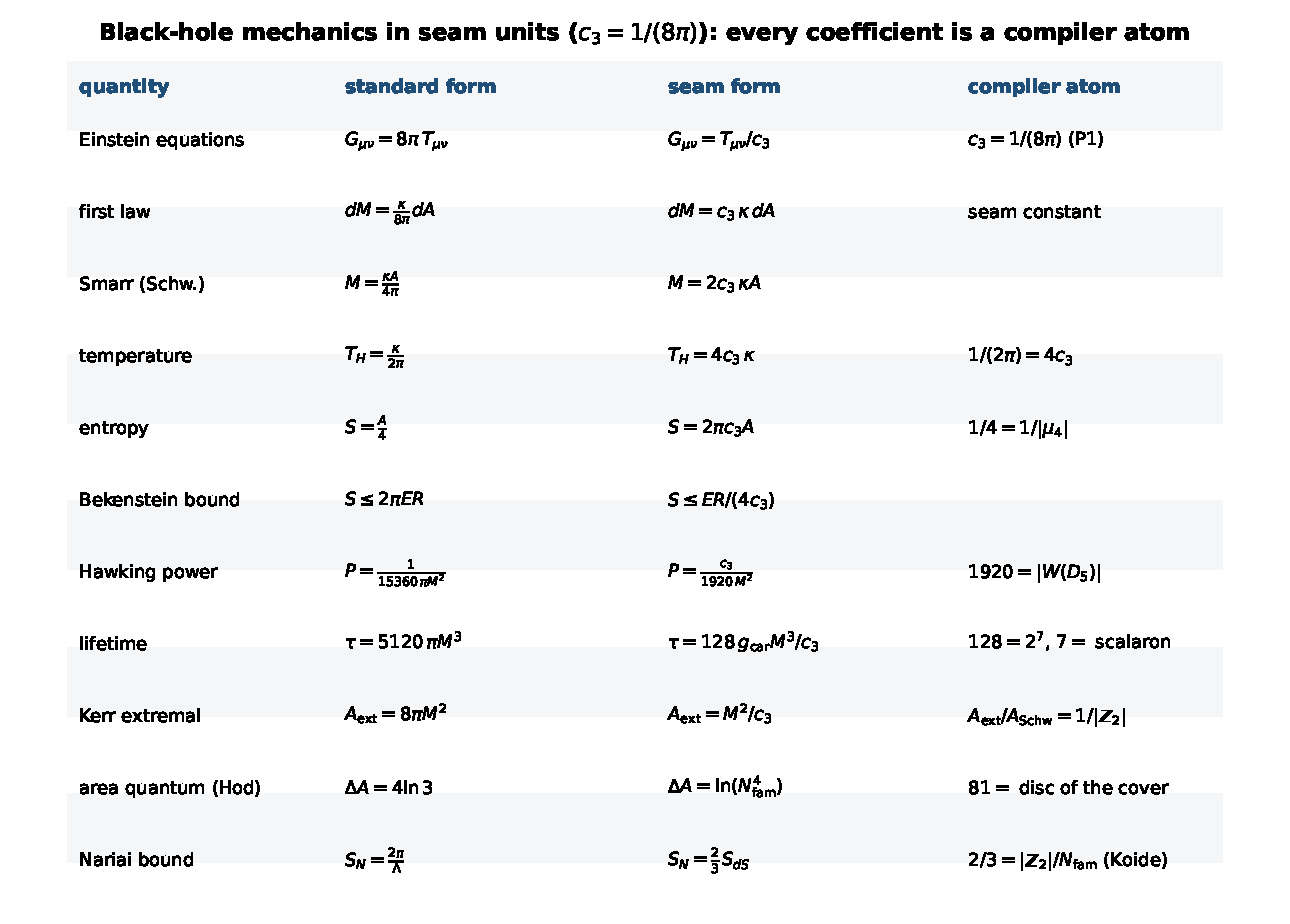
\includegraphics[width=0.9\linewidth]{figures/seam_units.pdf}
\caption{Black-hole mechanics in seam units: every classical coefficient is a compiler atom.
\veri{v101\_horizon\_anchor.py}}
\label{fig:seamunits}
\end{figure}

% =====================================================================
\section{Turnaround radius, gravitational waves, light}
% =====================================================================
\textbf{Bound structures.} In a $\Lambda$-universe the maximal bound radius is
$r_{\mathrm{ta}}(M)=\bigl(GM[\,2\pi e^{\ainv}/\Mbar]^2\bigr)^{1/3}$ --- halo, cluster, supercluster and
void scales follow from the $\Lambda$ closure with no new parameter. \mC

\textbf{Gravitational waves.} The low-curvature branch is $R+R^2$; the tensor graviton runs on the Lorentz
cone and the only extra mode (the scalaron, $M_{\mathrm{scal}}\approx3.06\times10^{13}$ GeV) is frozen for
astrophysical frequencies. Hence
\[
  \boxed{\ v_{\mathrm{GW}}=c\ }\qquad\text{(no measurable dispersion)}\qquad\mC,
\]
a clean falsifier: a genuine $v_{\mathrm{GW}}\ne c$ would break this gravity closure.

\textbf{Light.} TFPT does not predict the SI number $c$ (definitional); it predicts the \emph{universality
of the causal cone} --- RP $\to$ OS reconstruction $\to$ one Lorentzian cone shared by EM, gravity and
massless modes ($v_\gamma=v_g=c$, no native photon dispersion). What it \emph{does} compute is not a speed
shift but a polarisation rotation, cosmic birefringence
\[
  \boxed{\ \beta_{\mathrm{rad}}=\frac{u}{4\pi}\approx0.2424^\circ\ }\qquad\mE,
\]
from the same seed $u=\phi_0^{\mathrm{ret}}$ that fixes the Cabibbo angle, $\Omega_b$ and $\theta_{13}$.

% =====================================================================
\section{The local sibling: an EHT achromatic polarization intercept}
% =====================================================================
The cosmic birefringence $\beta_{\mathrm{rad}}$ is the \emph{asymptotic} (Thomson-limit) projection of the
determinant-line response; the \emph{local} projection onto the magnetised collar of a horizon-scale black
hole is a structured, achromatic residual rotation of the linear-polarization angle \veri{v203\_eht\_achromatic.py}
\[
  \beta_{\mathrm{BH}}(r)=\frac{Q_e^{\mathrm{eff}}(x)\,Q_m^{\mathrm{eff}}(x)}{256\pi^4\,r^2}
  =16\,\cthree^4\,\frac{Q_e^{\mathrm{eff}}Q_m^{\mathrm{eff}}}{r^2}
  =\frac{\delta_{\mathrm{top}}}{3}\,\frac{Q_e^{\mathrm{eff}}Q_m^{\mathrm{eff}}}{r^2},
\]
where the coupling $16\cthree^4=1/(256\pi^4)$ is fixed \emph{exactly} (\mE) --- the \emph{same} top-form
coefficient $\delta_{\mathrm{top}}=48\cthree^4=3/(256\pi^4)$ that controls the $\alpha$-kernel
precision-zone correction. There is \emph{no free coupling}: EHT-class polarimetry probes the same
admissibility data as the $\alpha$ row, only projected onto the local collar. What TFPT fixes is the
structured $1/r^2$ shape, the achromaticity, and the sign-flip under effective $E\!\cdot\!B$ reversal,
\emph{not} the amplitude $Q_e^{\mathrm{eff}}Q_m^{\mathrm{eff}}$ (an MHD/GR weight); the channel is therefore
typed \mC\ (shape/sign), not a parameter-free pixel prediction.
\par\smallskip\noindent\textbf{Dated kill test \mX.} Build the residual intercept
$\chi_0^{\mathrm{res}}=\chi_0^{\mathrm{obs}}-\chi_0^{\mathrm{GRMHD}}$ after honest GRMHD/synchrotron
subtraction; it must pass \emph{three independent nulls} --- frequency (achromatic, no $\lambda^2$ tail),
spatial ($1/r^2$ profile), and sign-flip (reverses under $E\!\cdot\!B$ reversal). A residual statistically
consistent with zero across the horizon-scale image, or failing any null, falsifies \emph{this channel}
(the compiler core is untouched). \emph{Scope:} the old UFE closed RN-type metric ($D/r^4$, regular cores,
shadow shift) is \emph{not} adopted --- it is superseded by the Nariai/seam$=$horizon readouts above
(\vref{v190}); only the polarization signature survives.

% =====================================================================
\section{Search targets (not claims)}
% =====================================================================
\begin{gapbox}[Audit-level search ansätze \mO]
\begin{itemize}\setlength\itemsep{2pt}
\item \textbf{Black-hole echoes:} any near-horizon echo amplitude ratio would be a natural transfer-rate
target, $\mathcal A_{n+1}/\mathcal A_n\lesssim(2/3)^6\approx0.0878$. A search ansatz, no prediction.
\item \textbf{Quantum recovery:} the Page-curve recovery kernel $I\sim(2/3)^{6n}$ is a falsifiable shape
if a boundary-recovery rate is ever measured.
\item \textbf{FRB repeaters:} fast-radio-burst repeaters are a \emph{preregistered search interface} for
the same boundary-recovery kernel (the frozen ratios $\{1,(2/3)^6,(1/3)^6\}$ and $\{1,(2/3)^3,(1/3)^3\}$),
\emph{not} a horizon claim and \emph{not} part of the verification ledger --- the work lives in
\texttt{experiments/frb-tfpt-signatures} with a frozen hypothesis file and surrogate-calibrated null tests;
current public data neither confirm nor refute the kernel (a clean null on echo ratios, a single
non-replicated window candidate). Hunting ground, not foundation.
\end{itemize}
\end{gapbox}

\begin{keybox}[Net]
All horizon formulas share the one seam normalisation $1/(2\pi)=4\cthree$. Black-hole, de Sitter and Unruh
temperatures, the Page time, scrambling, the Nariai bound, turnaround radii, $v_{\mathrm{GW}}=c$ and
birefringence are \emph{readouts of one seam constant} --- standard physics rewritten in TFPT units, with
two genuine compiler fingerprints ($1920=|W(D_5)|$ in Hawking power, $|\mu_4|=4$ in scrambling). No new
gravitational physics is claimed; the value of the reframe is that horizons stop being separate modules.
\end{keybox}

% =====================================================================
\section*{Appendix: computational verification}
% =====================================================================
The seam-unit identities of this note (the thermal grammar $\tfrac1{2\pi}{=}4\cthree$, the
power denominator $1920{=}|W(D_5)|$, the de Sitter entropy form, the Page fraction, the scrambling
$|\mu_4|{=}4$, and $\beta_{\rm rad}{=}\varphi_0^{\rm ret}/4\pi{=}0.2424^\circ$) are re-derived and machine-checked in
\texttt{verification/v8\_horizon.py}. Run \texttt{python verification/v8\_horizon.py} (needs
\texttt{mpmath}); it imports the same $\cthree{=}1/(8\pi)$ primitive as the rest of the suite. The
search-target ans\"atze remain \mO\ and are deliberately not part of the pass/fail checks.

\end{document}
